\documentclass[11pt,letterpaper,twocolumn]{article}

% ── Packages ──────────────────────────────────────────────
\usepackage[margin=0.85in]{geometry}
\usepackage[T1]{fontenc}
\usepackage{lmodern}
\usepackage{microtype}
\usepackage{graphicx}
\usepackage{xcolor}
\usepackage{tikz}
\usetikzlibrary{arrows.meta,positioning,shapes.geometric,fit,calc,
                 decorations.pathreplacing,backgrounds,patterns}
\usepackage{pgfplots}
\pgfplotsset{compat=1.18}
\usepackage{booktabs}
\usepackage{tabularx}
\usepackage{enumitem}
\usepackage{amsmath}
\usepackage{amssymb}
\usepackage{hyperref}
\usepackage{caption}
\usepackage{subcaption}
\usepackage{float}
\usepackage{multicol}
\usepackage{fancyhdr}
\usepackage{titlesec}

% ── Brand Colors ──────────────────────────────────────────
\definecolor{garnet}{HTML}{73000A}
\definecolor{rose}{HTML}{CC2E40}
\definecolor{atlantic}{HTML}{466A9F}
\definecolor{congaree}{HTML}{1F414D}
\definecolor{horseshoe}{HTML}{65780B}
\definecolor{grass}{HTML}{CED318}
\definecolor{honeycomb}{HTML}{A49137}
\definecolor{warmgrey}{HTML}{676156}
\definecolor{sandstorm}{HTML}{FFF2E3}
\definecolor{bk90}{HTML}{363636}
\definecolor{bk70}{HTML}{5C5C5C}
\definecolor{bk50}{HTML}{A2A2A2}
\definecolor{bk30}{HTML}{C7C7C7}
\definecolor{bk10}{HTML}{ECECEC}

% ── Hyperref config ───────────────────────────────────────
\hypersetup{
  colorlinks=true,
  linkcolor=garnet,
  citecolor=atlantic,
  urlcolor=congaree,
}

% ── Section styling ───────────────────────────────────────
\titleformat{\section}{\large\bfseries\color{garnet}}{\thesection}{0.8em}{}
\titleformat{\subsection}{\normalsize\bfseries\color{congaree}}{\thesubsection}{0.6em}{}
\titleformat{\subsubsection}{\normalsize\itshape\color{bk70}}{\thesubsubsection}{0.6em}{}

% ── Header / Footer ──────────────────────────────────────
\pagestyle{fancy}
\fancyhf{}
\fancyhead[L]{\small\color{bk70}From LLMs to Multi-Agent Systems}
\fancyhead[R]{\small\color{bk70}J.C.\ Vaught}
\fancyfoot[C]{\small\color{bk50}\thepage}
\renewcommand{\headrulewidth}{0.4pt}
\renewcommand{\headrule}{\hbox to\headwidth{\color{garnet}\leaders\hrule height \headrulewidth\hfill}}

% ── TikZ styles ───────────────────────────────────────────
\tikzset{
  agentbox/.style={
    rectangle, draw=#1, fill=#1!8, thick,
    minimum width=2.2cm, minimum height=0.8cm,
    font=\small\sffamily, align=center,
    inner sep=4pt
  },
  agentbox/.default=garnet,
  workerbox/.style={
    rectangle, draw=atlantic, fill=atlantic!8, thick,
    minimum width=1.8cm, minimum height=0.7cm,
    font=\small\sffamily, align=center,
    inner sep=3pt
  },
  tierbox/.style={
    rectangle, draw=#1, fill=#1!5, thick,
    minimum width=6.5cm, minimum height=1.0cm,
    font=\small\sffamily, align=center,
    inner sep=4pt
  },
  tierbox/.default=garnet,
  dataarrow/.style={
    -{Stealth[length=5pt]}, thick, color=#1
  },
  dataarrow/.default=bk70,
  brace/.style={
    decorate, decoration={brace, amplitude=6pt, raise=2pt}, thick, color=#1
  },
  brace/.default=bk50,
  labelnode/.style={
    font=\scriptsize\sffamily, color=bk70
  },
  % ── New styles for this document ──
  codebox/.style={rectangle, draw=bk70, fill=bk90, text=white,
    font=\ttfamily\small, inner sep=6pt, align=left, text width=#1},
  codebox/.default=6cm,
  sysprompt/.style={rectangle, draw=rose, dashed, fill=rose!5, thick,
    minimum width=2.0cm, minimum height=0.6cm,
    font=\small\sffamily, align=center, inner sep=3pt},
  tooldef/.style={rectangle, draw=atlantic, fill=atlantic!8, thick,
    minimum width=1.8cm, minimum height=0.6cm,
    font=\small\sffamily, align=center, inner sep=3pt},
  wrapperbox/.style={rectangle, draw=garnet, dashed, thick, fill=garnet!3,
    inner sep=8pt},
  pbar/.style={rectangle, draw=#1, fill=#1!30, thick,
    minimum height=0.3cm, font=\scriptsize\sffamily},
  pbar/.default=horseshoe,
  flag/.style={rectangle, draw=rose, fill=rose!15, thick,
    minimum width=0.8cm, minimum height=0.4cm,
    font=\tiny\sffamily\bfseries},
  failbox/.style={rectangle, draw=rose, fill=rose!10, thick,
    font=\small\sffamily, align=center, inner sep=4pt},
}

% ══════════════════════════════════════════════════════════
\title{\textcolor{garnet}{\textbf{From LLMs to Multi-Agent Systems}}\\[6pt]
  \large\textcolor{bk70}{A Progressive Guide to Agent Architectures}}
\author{J.C.\ Vaught\\
  \small University of South Carolina\\
  \small\texttt{jvaught@sc.edu}}
\date{\today}

\begin{document}
\maketitle
\thispagestyle{fancy}

% ── Abstract ──────────────────────────────────────────────
\begin{abstract}
\noindent
This document provides a comprehensive, progressive guide to multi-agent systems architectures, beginning with foundational concepts of large language models and advancing through increasingly complex architectures. Starting from single-agent systems, we progressively introduce slave hierarchies, orchestration patterns, and multi-layered hierarchies. The guide explores three agent execution models (streaming, batch, and parallel), multiple communication patterns (direct, file-mediated, and hybrid), and diverse control models (imperative, declarative, and hybrid). We examine orchestration cycles ranging from single-pass to iterative and reactive patterns, alongside system topologies including serial, parallel, and tree configurations. Central to this framework are four canonical patterns: pipeline, fan-out/fan-in, master-slave, and feedback loop architectures. Throughout, we provide practical guidance for selecting and combining patterns based on specific task characteristics, computational constraints, and system requirements.
\end{abstract}


% ── Part I: Foundation (Sections 1-3) ─────────────────────
%% sec_01_03_foundation.tex
%% Sections 1-3: What is an LLM? / AI-Assisted Coding / AI Coding Agent

\section{What Is an LLM?}\label{sec:llm}

\begin{figure*}[t]
\centering
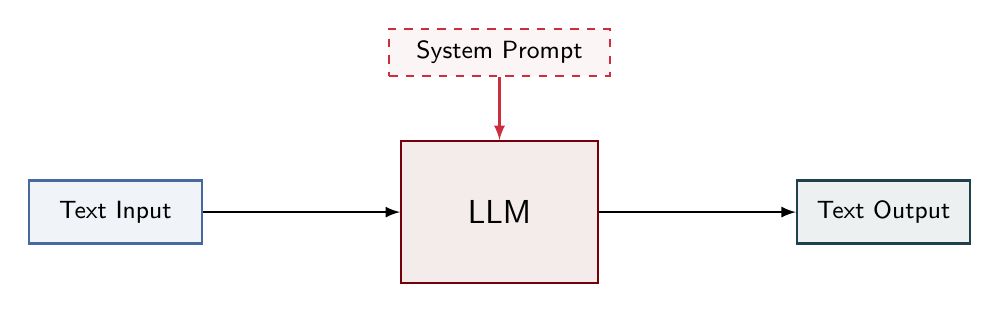
\begin{tikzpicture}[node distance=1.5cm and 2.5cm]
    \node[agentbox=atlantic] (textin1) {Text Input};
    \node[agentbox, right=of textin1, minimum width=2.5cm, minimum height=1.8cm] (llm1) {\large LLM};
    \node[agentbox=congaree, right=of llm1] (textout1) {Text Output};

    % System prompt above LLM
    \node[sysprompt, above=0.8cm of llm1, minimum width=2.8cm] (sysprompt1) {System Prompt};
    \draw[-latex, rose, thick] (sysprompt1) -- (llm1);

    % Arrows
    \draw[-latex, thick] (textin1) -- (llm1);
    \draw[-latex, thick] (llm1) -- (textout1);
\end{tikzpicture}
\caption{The fundamental LLM interface: text enters, the model processes it under constraints defined by an invisible system prompt, and text emerges. The model retains no information between conversations.}
\label{fig:llm_io}
\end{figure*}

Before understanding AI coding agents, we must understand the engine that powers them: the large language model, or LLM. Think of an LLM as a person who can talk but has no hands to manipulate objects, no persistent memory beyond the current conversation, and---usually---no eyes to see the world. This person has read vast amounts of text and learned patterns in language, allowing them to predict what words should come next in any conversation. When you send a message, the LLM generates a response based on everything said so far in the thread, then forgets the interaction the moment it ends.

The lack of memory is worth emphasizing because it contradicts many users' intuitions. When you close your chat with an LLM and open a new conversation tomorrow, the model has no recollection of what you discussed previously. There is no learning, no accumulation of experience, no relationship building. Each conversation is a blank slate. The LLM does not remember your name, your preferences, or the bug you fixed together last week. If the chatbot seems to remember you across sessions, that is the work of external systems maintaining conversation logs and feeding them back as context, not the model itself retaining information. This statelessness has profound implications for agents: without external memory systems, an agent cannot improve its performance on your specific codebase over time unless explicitly given access to logs, documentation, or other persistent records as input.

LLMs vary widely in capability. Some are small and fast but produce simple, sometimes unreliable output---like asking a novice for advice. Others are large and sophisticated, capable of nuanced reasoning and complex problem-solving, though they may take longer to respond. The key insight is that an LLM is fundamentally a prediction engine: given a sequence of text, it predicts the most likely continuation.

This size-capability tradeoff is central to practical deployment. A small model might have a few billion parameters and run efficiently on consumer hardware or respond in milliseconds via cloud APIs. Such models excel at simple tasks like code autocompletion, grammar correction, or answering factual questions. But ask them to debug a subtle concurrency issue or reason about trade-offs in system architecture, and their responses become shallow or incorrect. Conversely, a large model with hundreds of billions of parameters demonstrates impressive reasoning abilities---it can follow multi-step logic, recognize edge cases, and produce creative solutions. However, these capabilities come at a cost: substantial computational resources, higher API fees, and slower response times measured in seconds rather than milliseconds. Choosing the right model for a given task requires balancing accuracy, latency, and cost. In agent systems, where the LLM may be invoked hundreds of times to complete a single user request, these trade-offs compound quickly.

Some modern LLMs have gained ``eyes'' through multimodal capabilities, meaning they can accept images as input alongside text. This allows them to describe pictures, extract information from diagrams, or analyze visual data. However, the output remains purely textual. The LLM cannot draw, edit pixels, or manipulate files---it can only describe or reason about what it sees.

A critical but invisible component shapes every LLM interaction: the system prompt. Before you type a single word, the LLM has already received instructions from the system designer. This prompt might say ``you are a helpful assistant'' or ``you are a Python expert who writes concise code.'' The system prompt establishes the LLM's persona, constraints, and priorities. Users never see this text, but it influences every response -- often to my chagrin. A playful chatbot and a formal legal assistant may use the same underlying model, differing only in their system prompts.

To illustrate the power of system prompts, consider two interactions with the same LLM. First, with a system prompt reading ``You are a creative writing assistant who favors vivid imagery and emotional depth,'' a user asks, ``Describe a rainy day.'' The model might respond, ``The sky wept gray tears onto the cobblestones, each droplet a tiny percussion note in the city's melancholy symphony.'' Now give the same model a different system prompt: ``You are a technical weather analyst. Provide precise, factual descriptions.'' The identical user query yields, ``Precipitation of approximately 5 mm per hour with overcast cloud cover at 800 meters altitude, temperature 12 degrees Celsius, relative humidity 87 percent.'' Same model, same question, radically different output. The system prompt is not a minor detail---it is the lens through which the model interprets every user request. In agent systems, the system prompt often includes detailed instructions about when to call tools, how to format responses, and what safety checks to perform. A poorly crafted system prompt can render an otherwise capable model nearly useless for agent tasks.

We are simplifying dramatically here but for understanding agents, the essential picture suffices -- structured text goes in, the LLM processes it according to learned patterns and its system prompt, and structured text comes out.

\begin{figure*}[t]
\centering
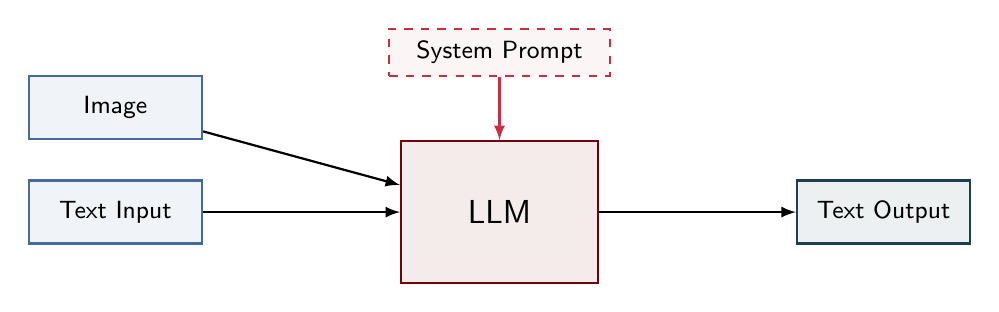
\begin{tikzpicture}[node distance=1.5cm and 2.5cm]
    \node[agentbox=atlantic] (image2) {Image};
    \node[agentbox=atlantic, below=0.5cm of image2] (textin2) {Text Input};
    \node[agentbox, right=of textin2, minimum width=2.5cm, minimum height=1.8cm] (llm2) {\large LLM};
    \node[agentbox=congaree, right=of llm2] (textout2) {Text Output};

    % System prompt above LLM
    \node[sysprompt, above=0.8cm of llm2, minimum width=2.8cm] (sysprompt2) {System Prompt};
    \draw[-latex, rose, thick] (sysprompt2) -- (llm2);

    % Arrows
    \draw[-latex, thick] (image2) -- (llm2);
    \draw[-latex, thick] (textin2) -- (llm2);
    \draw[-latex, thick] (llm2) -- (textout2);
\end{tikzpicture}
\caption{A multimodal LLM accepts images alongside text, but output remains purely textual. The model can describe, analyze, or reason about visual input---it cannot produce images.}
\label{fig:llm_multimodal}
\end{figure*}

\section{What Is AI-Assisted Coding?}\label{sec:autocomplete}

The simplest application of an LLM to software development is code autocompletion. Here, the LLM is given a system prompt that instructs it to act as a code completion engine: ``You are an expert programmer. Given partial code, predict the most likely continuation.'' The user types code into an editor, and whenever they pause, the LLM receives the text written so far and predicts what should come next. The prediction appears as gray ``ghost text'' that the user can accept with a keystroke or ignore by continuing to type.

This is a relatively narrow task. The LLM often has no access to other files in the project, cannot read documentation, and cannot execute or test the code it suggests. It relies entirely on patterns learned during training and the context provided in the current file. If the user has defined a function \texttt{calculate\_area} earlier in the file, the LLM may predict a call to that function when it seems appropriate. But the LLM is not searching the codebase or verifying correctness---it is simply continuing the established pattern.

Autocomplete represents the minimal intervention of AI in the coding process. The LLM does not take actions, make decisions, or interact with the development environment. It offers a single prediction, and the human decides whether to accept it. This simplicity is both a strength and a limitation. Autocomplete is fast, unobtrusive, and requires no additional infrastructure. But it cannot refactor code across multiple files, fetch API documentation, or debug a runtime error. For those tasks, we need something more capable: an agent.

\begin{figure*}[t]
\centering
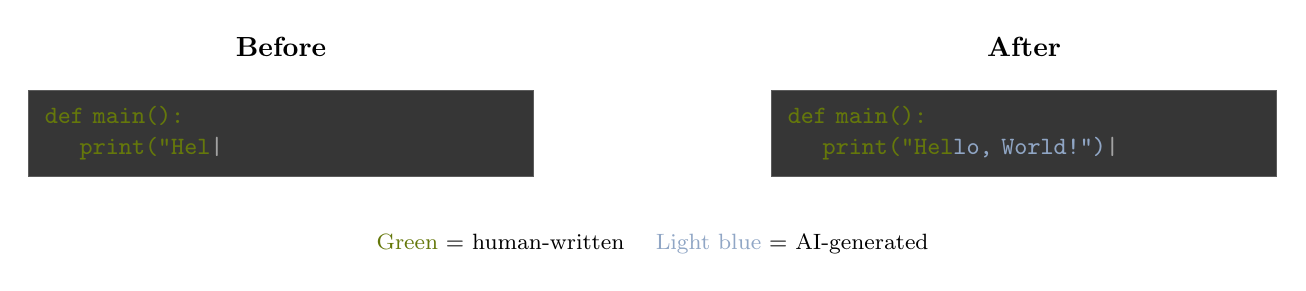
\begin{tikzpicture}[node distance=1.2cm]
    % LEFT PANEL: Before
    \node[codebox] (before) {%
        \textcolor{horseshoe}{\texttt{def main():}}\\
        \textcolor{horseshoe}{\texttt{~~~~print("Hel}}\textcolor{bk50}{|}%
    };
    \node[above=0.3cm of before, font=\bfseries] {Before};

    % RIGHT PANEL: After
    \node[codebox, right=3cm of before] (after) {%
        \textcolor{horseshoe}{\texttt{def main():}}\\
        \textcolor{horseshoe}{\texttt{~~~~print("Hel}}\textcolor{atlantic!60!white}{\texttt{lo, World!")}}\textcolor{bk50}{|}%
    };
    \node[above=0.3cm of after, font=\bfseries] {After};

    % Legend
    \node[below=0.6cm of $(before.south east)!0.5!(after.south west)$, font=\footnotesize, align=center] (legend) {%
        \textcolor{horseshoe}{Green} = human-written \quad
        \textcolor{atlantic!60!white}{Light blue} = AI-generated%
    };
\end{tikzpicture}
\caption{AI-assisted code completion: the user types partial code, the LLM predicts the continuation, and the suggestion appears inline. The model operates purely on visible context with no access to files, tools, or execution environments.}
\label{fig:autocomplete}
\end{figure*}

\section{What Is an AI Coding Agent?}\label{sec:agent}

An agent transforms an LLM from a passive predictor into an active collaborator. The LLM itself does not change---it still receives text and produces text. What changes is the infrastructure wrapped around it. A coding agent consists of the LLM plus a wrapper program that orchestrates interactions between the model, the development environment, and the user.

The wrapper provides the LLM with two critical additions beyond the system prompt: tool definitions and an execution environment. Tool definitions describe actions the agent can take, such as ``read a file,'' ``run a command,'' or ``search the codebase.'' Each definition specifies the tool's name, parameters, and purpose. The LLM does not directly execute these tools---it cannot. Instead, when the LLM determines that a tool would help answer the user's request, it outputs a structured tool call in its response. The wrapper program parses this output, detects the tool call, executes the requested action in the real environment, and feeds the result back to the LLM as new context.

This creates a loop. The user sends a request. The LLM considers the request alongside its system prompt, available tools, and conversation history, then produces a response. If the response contains a tool call, the wrapper executes it, appends the result to the conversation, and invokes the LLM again. The LLM now has additional information and can either call another tool or provide a final answer. This cycle continues until the LLM produces a response with no tool calls, signaling that the task is complete.

The wrapper exerts control over what the agent can and cannot do. It decides which tools are available, enforces safety constraints (preventing destructive operations without confirmation), and manages the user interface. If the LLM requests a tool that does not exist or provides invalid parameters, the wrapper catches the error and may return a message to the LLM explaining the problem. The wrapper also handles concurrency, timeouts, and resource limits---concerns far beyond the LLM's domain.

From the user's perspective, the agent appears to act autonomously. They might ask, ``Fix the bug in \texttt{parser.py},'' and observe the agent reading the file, analyzing the code, running tests, editing the file, and re-running tests to confirm the fix. But this autonomy is an illusion choreographed by the wrapper. The LLM is still only predicting text, albeit text that encodes tool calls. The wrapper translates those predictions into real-world actions.

This architecture is extrmeely powerful. By giving the LLM access to file systems, compilers, debuggers, version control, and external APIs through tool calls, the agent can perform tasks that would be impossible for raw autocompletion. Yet it inherits all the LLM's limitations: no persistent memory across sessions, no ability to learn from mistakes without retraining, and occasional lapses in reasoning. The agent is not intelligent in a human sense---it is an LLM augmented with the ability to manipulate its environment, guided by a carefully crafted system prompt and constrained by the tools its wrapper provides.

\begin{figure*}[t]
\centering
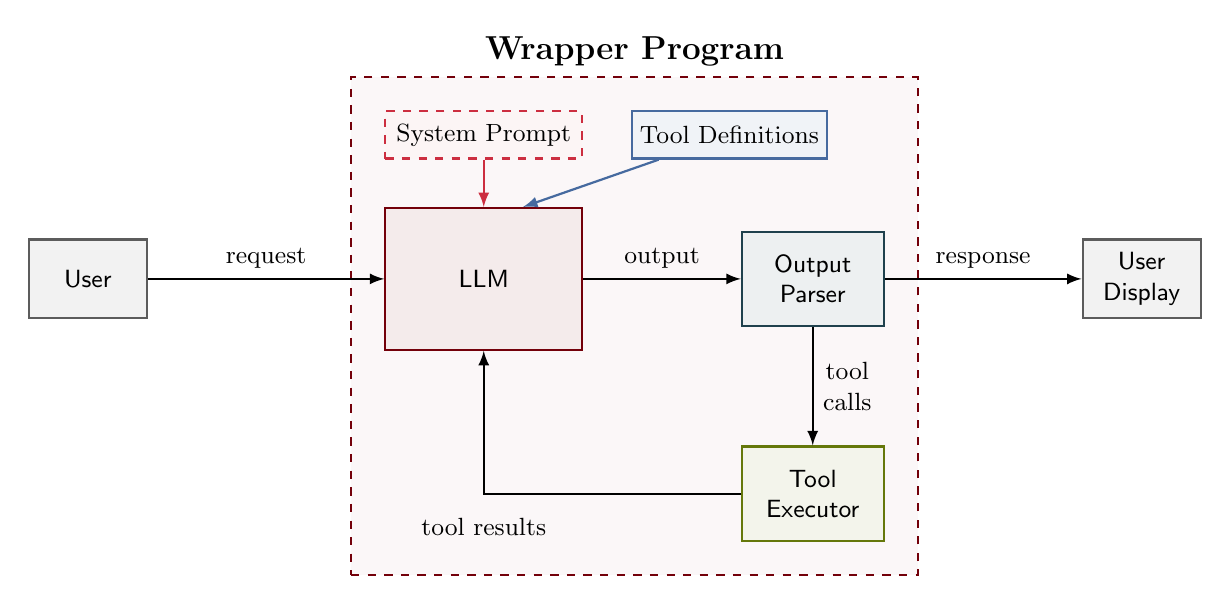
\begin{tikzpicture}[node distance=1.2cm and 2cm, >={Latex[length=2mm]}]
    % User node
    \node[agentbox=bk70, minimum width=1.5cm, minimum height=1cm] (user) {User};

    % LLM node
    \node[agentbox, right=3cm of user, minimum width=2.5cm, minimum height=1.8cm] (llm) {LLM};

    % System prompt directly above LLM, tool definitions to its right
    \node[sysprompt, above=0.6cm of llm, minimum width=2.5cm, font=\small] (sysprompt) {System Prompt};
    \node[tooldef, right=0.6cm of sysprompt, minimum width=2.2cm, font=\small] (tooldef) {Tool Definitions};
    \draw[-latex, rose, thick] (sysprompt) -- (llm);
    \draw[-latex, atlantic, thick] (tooldef) -- ([xshift=0.5cm]llm.north);

    % Output parser
    \node[agentbox=congaree, right=of llm, minimum width=1.8cm, minimum height=1.2cm] (parser) {Output\\Parser};

    % Tool executor (below parser)
    \node[agentbox=horseshoe, below=1.5cm of parser, minimum width=1.8cm, minimum height=1.2cm] (executor) {Tool\\Executor};

    % User display (outside wrapper)
    \node[agentbox=bk70, right=2.5cm of parser, minimum width=1.5cm, minimum height=1cm] (display) {User\\Display};

    % Wrapper program container (behind all nodes)
    \begin{scope}[on background layer]
      \node[wrapperbox, fit=(sysprompt)(tooldef)(llm)(parser)(executor), inner sep=12pt] (wrapper) {};
    \end{scope}
    \node[above=0cm of wrapper.north, font=\bfseries\large] {Wrapper Program};

    % Arrows
    \draw[-latex, thick] (user) -- (llm) node[midway, above, font=\small] {request};
    \draw[-latex, thick] (llm) -- (parser) node[midway, above, font=\small] {output};
    \draw[-latex, thick] (parser) -- (executor) node[midway, right, font=\small, align=center] {tool\\calls};
    \draw[-latex, thick] (parser) -- (display) node[midway, above, font=\small] {response};

    % Feedback loop: left to under LLM, then up
    \draw[-latex, thick] (executor.west) -- (executor.west -| llm.south) -- (llm.south) node[pos=-0.1, below, font=\small] {tool results};
\end{tikzpicture}
\caption{Architecture of an AI coding agent. The wrapper program mediates all interactions between the user and the LLM, parsing outputs to detect tool calls, executing those calls in the development environment, and feeding results back to the model. The LLM operates under constraints defined by its system prompt and the tools made available by the wrapper.}
\label{fig:agent_architecture}
\end{figure*}


% ── Part II: Workflows (Sections 4-6) ─────────────────────
%% Sections 4, 5, 6: Agent Workflow Patterns

\section{Agent Workflow --- Streaming Execution}\label{sec:streaming}

In a streaming execution model, the wrapper monitors the LLM's output token-by-token as it is generated. As soon as a complete tool call is detected in the stream, the wrapper immediately pauses the LLM's generation, executes the tool, appends the result to the conversation context, and resumes generation. This cycle repeats until the LLM emits a terminate signal indicating no further actions are required.

The primary advantage of streaming execution is responsiveness. Users see output appearing in real time rather than waiting for a complete response. Tools fire as soon as they are needed, minimizing latency between decision and action. This creates a more interactive experience where intermediate results can inform subsequent reasoning steps without waiting for the entire generation to complete.

However, streaming execution requires more sophisticated infrastructure. The wrapper must parse incomplete output, maintain state across pause-resume cycles, and handle potential errors in partially generated tool calls. The LLM must also be capable of resuming generation coherently after external results are injected mid-stream.

Figure~\ref{fig:streaming} illustrates this workflow. The LLM generates output continuously, monitored for tool calls. Upon detection, execution is handed off to the tool, results are appended, and generation resumes. The process terminates only when the LLM explicitly signals completion.

\section{Agent Workflow --- Batch Execution}\label{sec:batch}

Batch execution follows a simpler but less responsive pattern. The LLM generates its entire response in one pass until it naturally stops. Only then does the wrapper parse the complete output, extract all tool calls present, and execute them serially one after another. All tool results are collected and fed back to the LLM simultaneously, prompting a new generation cycle. This process repeats until the LLM produces output with no tool calls, indicating task completion.

This is the classic chatbot model familiar from interactive coding assistants: the agent writes code, attempts to run it, receives error messages, and tries again. Batch execution is significantly simpler to implement than streaming because it requires no real-time parsing or state management. The wrapper operates on complete, well-formed outputs and can use standard parsing techniques.

The trade-off is latency. Users must wait for the entire generation to complete before any tools execute, and all tools must finish before the next reasoning step begins. For complex tasks requiring multiple tool invocations, this can result in noticeable delays between observable progress. However, for tasks where tool calls are infrequent or where thoughtful planning precedes action, batch execution provides a robust and maintainable architecture.

Figure~\ref{fig:batch} shows the batch workflow. The LLM produces complete output, which is parsed to extract all tool calls. These are executed serially, producing a combined result set that is fed back to the LLM to trigger the next generation cycle.

\section{Agent Workflow --- Parallel Execution}\label{sec:parallel_exec}

Parallel execution extends the batch model by introducing concurrency. Each tool call generated by the LLM can carry a flag indicating whether it can execute in parallel with other operations or requires blocking synchronous execution. When the LLM generates a tool call marked for parallel execution, the wrapper launches it asynchronously and allows the LLM to continue generating additional output or tool calls. When a non-parallel tool call is encountered or the LLM emits a terminate signal, the wrapper stops, waits for all pending parallel operations to complete, executes any blocking tool, and feeds all accumulated results back to the LLM.

This architecture combines the responsiveness of streaming execution with the throughput advantages of concurrency. Multiple independent operations—such as reading several files, running tests, or querying external APIs—can proceed simultaneously without blocking each other or the LLM's reasoning process. Critical operations that depend on prior results or require exclusive access to resources can still be executed synchronously to maintain correctness.

The complexity lies in managing parallel task lifetimes, handling errors from concurrent operations, and ensuring deterministic behavior when multiple results arrive out of order. The wrapper must track which parallel operations are outstanding, aggregate their results, and present them coherently to the LLM. The LLM itself must understand which operations can safely run concurrently and which require sequential ordering.

Figure~\ref{fig:parallel_workflow} illustrates this model. Tools marked with a parallel flag execute concurrently while generation continues. A synchronization barrier is inserted before any blocking tool, ensuring all prior parallel operations complete before the blocking operation begins. All results are then returned to the LLM together, maintaining a consistent view of the execution state.

\begin{figure*}[t]
\centering
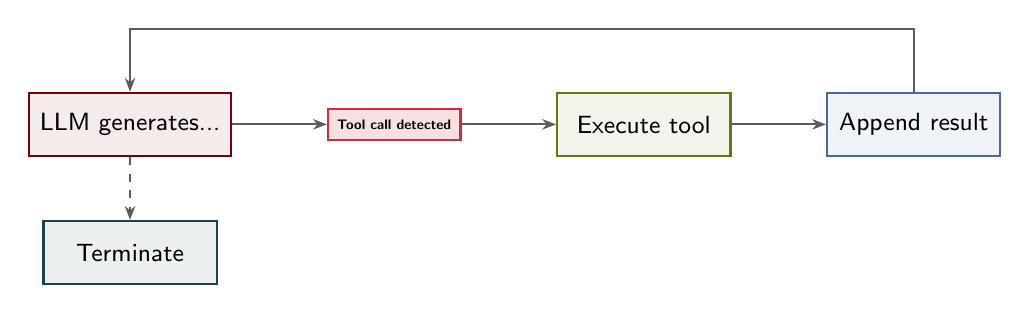
\begin{tikzpicture}[node distance=1.5cm and 1.2cm]

\node[agentbox] (llm1) {LLM generates...};
\node[flag, right=of llm1] (detect) {Tool call detected};
\node[agentbox=horseshoe, right=of detect] (exec) {Execute tool};
\node[agentbox=atlantic, right=of exec] (append) {Append result};

\node[agentbox=congaree, below=0.8cm of llm1] (term1) {Terminate};

\draw[dataarrow] (llm1) -- (detect);
\draw[dataarrow] (detect) -- (exec);
\draw[dataarrow] (exec) -- (append);
\draw[dataarrow] (append.north) -- ++(0,0.8) -| (llm1.north);
\draw[dataarrow, dashed] (llm1) -- (term1);

\end{tikzpicture}
\caption{Streaming execution workflow. The LLM generates output incrementally; as soon as a tool call is detected, execution pauses, the tool runs, results are appended, and generation resumes. The process repeats until the LLM emits a terminate signal.}
\label{fig:streaming}
\end{figure*}

\begin{figure*}[t]
\centering
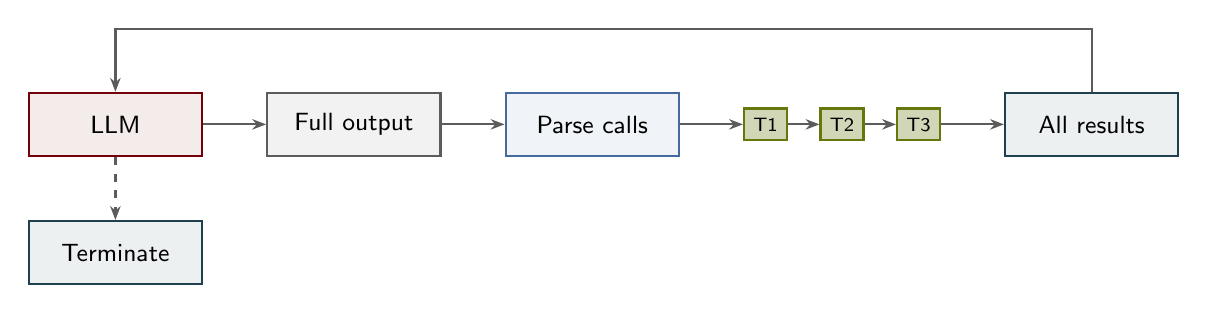
\begin{tikzpicture}[node distance=0.8cm and 0.8cm]

\node[agentbox] (llm2) {LLM};
\node[agentbox=bk70, right=of llm2] (output) {Full output};
\node[agentbox=atlantic, right=of output] (parse) {Parse calls};
\node[pbar, right=of parse] (t1) {T1};
\node[pbar, right=0.4cm of t1] (t2) {T2};
\node[pbar, right=0.4cm of t2] (t3) {T3};
\node[agentbox=congaree, right=of t3] (allres) {All results};

% Terminate under LLM
\node[agentbox=congaree, below=0.8cm of llm2] (term2) {Terminate};
\draw[dataarrow, dashed] (llm2) -- (term2);

% Main flow
\draw[dataarrow] (llm2) -- (output);
\draw[dataarrow] (output) -- (parse);
\draw[dataarrow] (parse) -- (t1);
\draw[dataarrow] (t1) -- (t2);
\draw[dataarrow] (t2) -- (t3);
\draw[dataarrow] (t3) -- (allres);
\draw[dataarrow] (allres.north) -- ++(0,0.8) -| (llm2.north);

\end{tikzpicture}
\caption{Batch execution workflow. The LLM generates a complete response, tool calls are parsed and executed serially (T1, T2, T3), and all results are fed back to trigger the next reasoning cycle.}
\label{fig:batch}
\end{figure*}

\begin{figure*}[t]
\centering
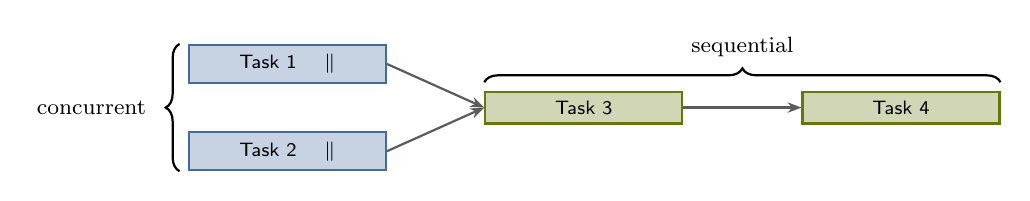
\begin{tikzpicture}[node distance=1.2cm and 1.8cm]

% Parallel tasks
\node[pbar=atlantic, minimum width=2.5cm] (t1) {Task 1 \quad $\parallel$};
\node[pbar=atlantic, minimum width=2.5cm, below=0.6cm of t1] (t2) {Task 2 \quad $\parallel$};

% Serial tasks
\node[pbar=horseshoe, minimum width=2.5cm, right=2.5cm of $(t1)!0.5!(t2)$] (t3) {Task 3};
\node[pbar=horseshoe, minimum width=2.5cm, right=1.5cm of t3] (t4) {Task 4};

% Arrows from parallel into serial
\draw[dataarrow] (t1.east) -- (t3.west);
\draw[dataarrow] (t2.east) -- (t3.west);
\draw[dataarrow] (t3) -- (t4);

% Annotations
\draw[thick, decorate, decoration={brace, amplitude=5pt, mirror, raise=3pt}]
  (t1.north west) -- (t2.south west)
  node[midway, left=0.4cm, font=\footnotesize, align=center] {concurrent};
\draw[thick, decorate, decoration={brace, amplitude=5pt, raise=3pt}]
  (t3.north west) -- (t4.north east)
  node[midway, above=0.3cm, font=\footnotesize, align=center] {sequential};

\end{tikzpicture}
\caption{Parallel execution: tasks marked $\parallel$ run concurrently. Once both complete, subsequent tasks execute sequentially. The agent decides which tasks are independent and can safely overlap.}
\label{fig:parallel_workflow}
\end{figure*}


% ── Part III: Sub-Agents & Management (Sections 7-11) ─────
%% Section 7: What Is a Sub-Agent?
\section{What Is a Sub-Agent?}\label{sec:subagent}

A sub-agent is architecturally identical to the agent described in Section~\ref{sec:agent}. It possesses the same core components: an LLM capable of reasoning and tool use, a system prompt that defines its behavior, and access to tools for interacting with the environment. The critical distinction is not in its internal structure but in its invocation: a sub-agent is called by another agent rather than directly by a human user.

This architectural equivalence allows for significant flexibility in deployment. A sub-agent may run the same model as its parent, but more commonly it uses a different model optimized for its specialized task. A parent agent handling general orchestration might use a large, capable model, while delegating narrowly-scoped work to sub-agents running smaller, faster, or domain-tuned models. Similarly, the system prompt of a sub-agent is typically specialized for a particular domain—code refactoring, test execution, documentation generation, data validation—rather than the general-purpose instructions given to a primary agent.

Tool access is also scoped to the sub-agent's responsibilities. Where a parent agent might have access to the full suite of development tools, a sub-agent focused on testing might be restricted to test execution frameworks and assertion libraries. This scoping reduces complexity, improves safety, and allows the sub-agent's reasoning to focus on a well-defined problem space.

\begin{figure*}[t]
\centering
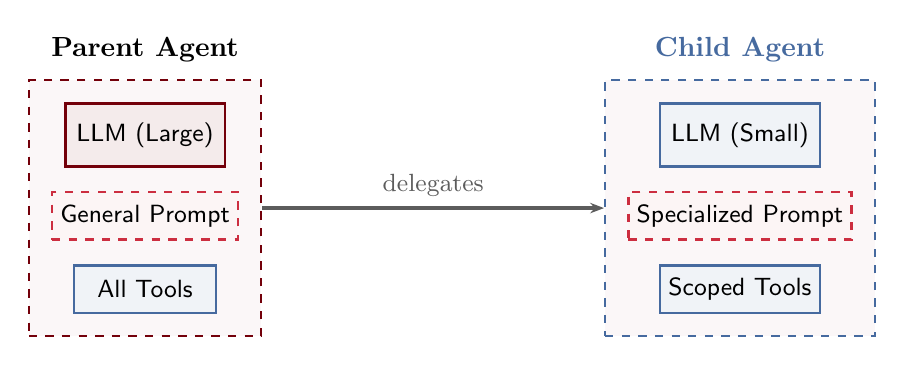
\begin{tikzpicture}[node distance=0.3cm and 1.5cm]

% Parent Agent
\node[agentbox, minimum width=2cm] (parent-llm) {LLM (Large)};
\node[sysprompt, below=of parent-llm] (parent-prompt) {General Prompt};
\node[tooldef, below=of parent-prompt] (parent-tools) {All Tools};
% Child Agent
\node[agentbox=atlantic, minimum width=2cm, right=5.5cm of parent-llm] (child-llm) {LLM (Small)};
\node[sysprompt, below=of child-llm] (child-prompt) {Specialized Prompt};
\node[tooldef, below=of child-prompt] (child-tools) {Scoped Tools};

% Wrapper boxes on background layer
\begin{scope}[on background layer]
  \node[wrapperbox, draw=garnet, dashed, fit=(parent-llm)(parent-prompt)(parent-tools), inner sep=8pt] (parent-wrapper) {};
  \node[wrapperbox, draw=atlantic, dashed, fit=(child-llm)(child-prompt)(child-tools), inner sep=8pt] (child-wrapper) {};
\end{scope}

\node[above=0.1cm of parent-wrapper.north, font=\bfseries] {Parent Agent};
\node[above=0.1cm of child-wrapper.north, font=\bfseries, text=atlantic] {Child Agent};

% Arrow
\draw[dataarrow, line width=1.5pt] (parent-wrapper.east) -- (child-wrapper.west)
  node[midway, above, font=\small] {delegates};

\end{tikzpicture}
\caption{A sub-agent shares the same architecture as a standard agent (Section~\ref{sec:agent}) but differs in its model selection, system prompt specialization, and tool access scope.}
\label{fig:subagent}
\end{figure*}

%% Section 8: Sub-Agent Workflow
\section{Sub-Agent Workflow}\label{sec:subagent_workflow}

The lifecycle of a sub-agent begins when the parent agent constructs a detailed prompt describing the task to be performed. This prompt is delivered to the sub-agent, where it is combined with the sub-agent's own system prompt to form the complete context for execution. The system prompt provides domain expertise and behavioral constraints, while the parent's prompt supplies the specific task instance and any relevant data.

Once initialized, the sub-agent executes its task using any of the three reasoning patterns described in Sections~\ref{sec:streaming}--\ref{sec:parallel_exec}. A sub-agent for code refactoring might use streaming mode to interactively rewrite functions, a testing sub-agent might operate in batch mode to execute a suite and compile results, and a documentation sub-agent might parallelize the generation of API reference sections. The choice of execution pattern is determined by the sub-agent's design and the nature of its task, not by the fact that it is a sub-agent.

Upon completion, the sub-agent returns control to its parent. The exact form of this return varies: the sub-agent may include its result directly in a completion message, write outputs to disk and signal completion, or employ a hybrid approach. Regardless of the mechanism, the parent receives notification that the sub-agent has finished and can then integrate the result into its own reasoning process. This integration might involve validating the sub-agent's output, using it as input to another sub-agent, or incorporating it into a final deliverable for the user.

\begin{figure*}[t]
\centering
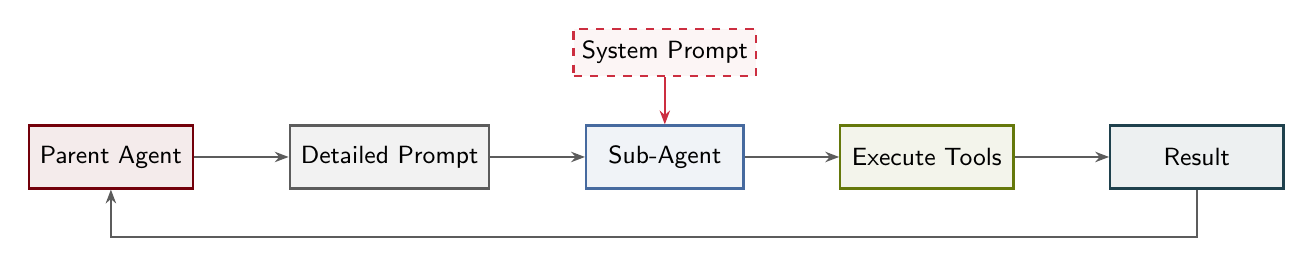
\begin{tikzpicture}[node distance=0.8cm and 1.2cm]

% Horizontal flow
\node[agentbox, minimum width=2cm] (parent) {Parent Agent};
\node[agentbox=bk70, right=of parent] (prompt) {Detailed Prompt};
\node[agentbox=atlantic, right=of prompt, minimum width=2cm] (subllm) {Sub-Agent};
\node[agentbox=horseshoe, right=of subllm] (exec) {Execute Tools};
\node[agentbox=congaree, right=of exec] (result) {Result};

% System prompt feeding into sub-agent from above
\node[sysprompt, above=0.6cm of subllm] (sysp) {System Prompt};
\draw[dataarrow=rose] (sysp) -- (subllm);


% Main flow arrows
\draw[dataarrow] (parent) -- (prompt);
\draw[dataarrow] (prompt) -- (subllm);
\draw[dataarrow] (subllm) -- (exec);
\draw[dataarrow] (exec) -- (result);

% Loop back to parent
\draw[dataarrow] (result.south) -- ++(0,-0.6) -| (parent.south);

\end{tikzpicture}
\caption{Sub-agent lifecycle. The parent crafts a detailed prompt, the sub-agent combines it with its own system prompt, executes tools using any execution pattern, and returns results to the parent.}
\label{fig:subagent_lifecycle}
\end{figure*}

%% Section 9: How Do We Manage Sub-Agents?
\section{How Do We Manage Sub-Agents?}\label{sec:manage}

The master-slave pattern provides the foundation for managing multiple sub-agents. In this architecture, a master agent serves as the coordinator, responsible for decomposing complex work into discrete tasks and distributing those tasks to specialized slave sub-agents. The master does not perform the work itself; instead, it coordinates, tracks progress, and synthesizes results.

A critical element of this pattern is the completion signal. Regardless of the communication mechanism employed—direct return, file-mediated output, or hybrid approaches—every slave must signal when it has finished its assigned task. This signal may be as simple as a boolean flag or as rich as a structured status message, but its presence is non-negotiable. Without reliable completion signals, the master cannot accurately track system state or make informed decisions about subsequent actions.

The master maintains state about the entire pool of slaves. This state includes which slaves are currently executing, which have completed their tasks, what results have been received, and what work remains to be distributed. When a slave signals completion, the master updates its internal model, evaluates whether dependencies have been satisfied, and determines the next steps. This might involve launching additional slaves to handle newly unblocked tasks, aggregating results from completed slaves to produce a final output, or escalating issues when a slave reports failure.

\begin{figure*}[t]
\centering
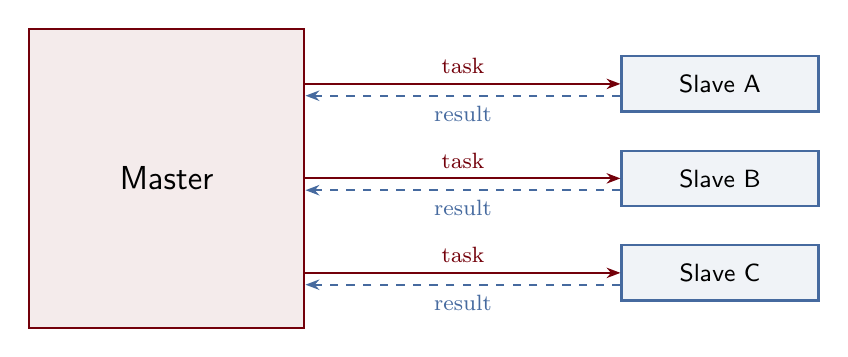
\begin{tikzpicture}[node distance=0.6cm]

% Master on the left
\node[agentbox=garnet, minimum width=3.5cm, minimum height=3.8cm] (master) {\large Master};

% Workers stacked on the right
\node[workerbox, right=4cm of master, yshift=1.2cm, minimum width=2.5cm] (w1) {Slave A};
\node[workerbox, right=4cm of master, yshift=0.0cm, minimum width=2.5cm] (w2) {Slave B};
\node[workerbox, right=4cm of master, yshift=-1.2cm, minimum width=2.5cm] (w3) {Slave C};

% Task arrows: master to workers (solid, straight horizontal)
\draw[dataarrow=garnet] (master.east |- w1) -- (w1.west)
  node[midway, above, font=\footnotesize] {task};
\draw[dataarrow=garnet] (master.east |- w2) -- (w2.west)
  node[midway, above, font=\footnotesize] {task};
\draw[dataarrow=garnet] (master.east |- w3) -- (w3.west)
  node[midway, above, font=\footnotesize] {task};

% Result arrows: workers to master (dashed, offset slightly below)
\draw[dataarrow=atlantic, dashed] ([yshift=-0.15cm]w1.west) -- ([yshift=-0.15cm]master.east |- w1)
  node[midway, below, font=\footnotesize] {result};
\draw[dataarrow=atlantic, dashed] ([yshift=-0.15cm]w2.west) -- ([yshift=-0.15cm]master.east |- w2)
  node[midway, below, font=\footnotesize] {result};
\draw[dataarrow=atlantic, dashed] ([yshift=-0.15cm]w3.west) -- ([yshift=-0.15cm]master.east |- w3)
  node[midway, below, font=\footnotesize] {result};

\end{tikzpicture}
\caption{The master-slave pattern. The master assigns tasks to slaves via straight delegation (solid) and receives results back (dashed). Each slave operates independently with its own context.}
\label{fig:orchestrator_workers}
\end{figure*}

%% Section 10: Communication Patterns
\section{Communication Patterns}\label{sec:comm}

The communication pattern between master and slave determines how results flow back to the master. Three patterns dominate in practice, each suited to different types of tasks and output characteristics.

\textbf{Direct return} embeds the result directly in the completion message. This pattern is appropriate when the master requires the slave's answer to make an immediate decision. A testing slave might return a simple pass/fail verdict, an installation slave might report success or error codes, and a query slave might return a small dataset or configuration value. The advantage is immediacy and simplicity: the master receives everything it needs in a single message. The disadvantage is scalability: large results bloat messages and may exceed protocol limits.

\textbf{File-mediated communication} separates the completion signal from the result. The slave writes its output to disk—a dataset, a rendered image, a binary artifact, newly generated source files—and then sends a minimal completion message to the master. The master can then read the file if and when it needs the data. This pattern is essential for large outputs that would be impractical to transmit inline. It also naturally handles side effects: when a code generation slave produces new source files, those files are the deliverable, not a message describing them. The slave still sends a completion flag to notify the master that the work is done, but the substantive output lives on disk.

\textbf{Hybrid communication}, the most common pattern in production systems, combines both approaches. The slave writes detailed artifacts to disk and simultaneously returns a summary in its completion message. A test runner might write full logs and stack traces to a file while returning "14 passed, 2 failed" to the master. A data processing slave might serialize a large DataFrame to disk while returning basic statistics (row count, schema, validation errors) inline. This gives the master enough information to make decisions without forcing it to parse large files, while preserving complete outputs for debugging, auditing, or downstream consumption.

\begin{figure*}[t]
\centering
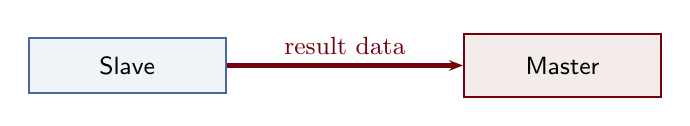
\begin{tikzpicture}[node distance=1.2cm and 2.5cm]

% Worker and Master
\node[workerbox, minimum width=2.5cm] (w1) {Slave};
\node[agentbox, right=3cm of w1, minimum width=2.5cm] (m1) {Master};

% Single thick arrow with result
\draw[dataarrow=garnet, line width=1.5pt] (w1) -- (m1)
  node[midway, above, font=\small] {result data};

\end{tikzpicture}
\caption{Direct return: the worker embeds its result in the completion message. Simple and immediate, suited for small results like pass/fail verdicts or status codes.}
\label{fig:comm_direct}
\end{figure*}

\begin{figure*}[t]
\centering
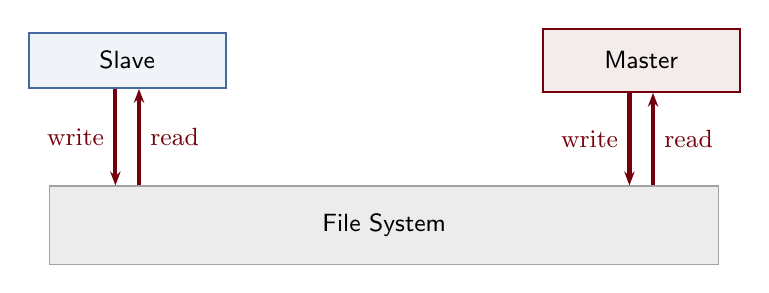
\begin{tikzpicture}[node distance=1.2cm and 2cm]

% Worker and Master on top
\node[workerbox, minimum width=2.5cm] (w2) {Slave};
\node[agentbox, right=4cm of w2, minimum width=2.5cm] (m2) {Master};

% Wide file system bar underneath
\node[rectangle, draw=bk50, fill=bk10, minimum width=8.5cm, minimum height=1cm,
  below=1.2cm of $(w2.south)!0.5!(m2.south)$, font=\small\sffamily] (file) {File System};

% Worker read/write (solid, bidirectional)
\draw[dataarrow=garnet, line width=1.5pt] ([xshift=-0.15cm]w2.south) -- ([xshift=-0.15cm]w2.south |- file.north)
  node[midway, left, font=\small] {write};
\draw[dataarrow=garnet, line width=1.5pt] ([xshift=0.15cm]w2.south |- file.north) -- ([xshift=0.15cm]w2.south)
  node[midway, right, font=\small] {read};

% Master read/write (solid, bidirectional)
\draw[dataarrow=garnet, line width=1.5pt] ([xshift=-0.15cm]m2.south) -- ([xshift=-0.15cm]m2.south |- file.north)
  node[midway, left, font=\small] {write};
\draw[dataarrow=garnet, line width=1.5pt] ([xshift=0.15cm]m2.south |- file.north) -- ([xshift=0.15cm]m2.south)
  node[midway, right, font=\small] {read};

\end{tikzpicture}
\caption{File-mediated: the worker writes output to a shared file system and sends only a completion signal. The master reads the file when needed. Suited for large artifacts, binaries, or generated source files.}
\label{fig:comm_file}
\end{figure*}

\begin{figure*}[t]
\centering
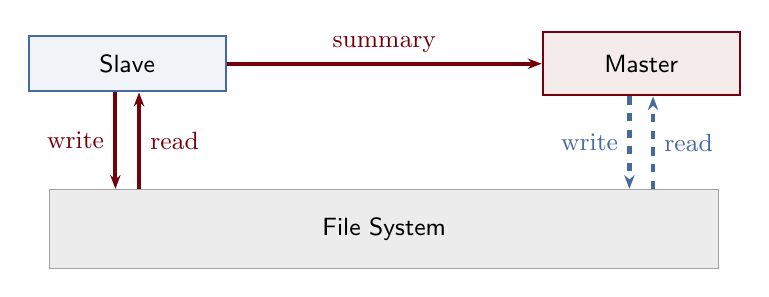
\begin{tikzpicture}[node distance=1.2cm and 2cm]

% Worker and Master on top
\node[workerbox, minimum width=2.5cm] (w3) {Slave};
\node[agentbox, right=4cm of w3, minimum width=2.5cm] (m3) {Master};

% Wide file system bar underneath
\node[rectangle, draw=bk50, fill=bk10, minimum width=8.5cm, minimum height=1cm,
  below=1.2cm of $(w3.south)!0.5!(m3.south)$, font=\small\sffamily] (file3) {File System};

% Worker read/write (solid)
\draw[dataarrow=garnet, line width=1.5pt] ([xshift=-0.15cm]w3.south) -- ([xshift=-0.15cm]w3.south |- file3.north)
  node[midway, left, font=\small] {write};
\draw[dataarrow=garnet, line width=1.5pt] ([xshift=0.15cm]w3.south |- file3.north) -- ([xshift=0.15cm]w3.south)
  node[midway, right, font=\small] {read};

% Master read/write (dashed)
\draw[dataarrow=atlantic, dashed, line width=1.5pt] ([xshift=-0.15cm]m3.south) -- ([xshift=-0.15cm]m3.south |- file3.north)
  node[midway, left, font=\small] {write};
\draw[dataarrow=atlantic, dashed, line width=1.5pt] ([xshift=0.15cm]m3.south |- file3.north) -- ([xshift=0.15cm]m3.south)
  node[midway, right, font=\small] {read};

% Summary arrow directly to master
\draw[dataarrow=garnet, line width=1.5pt] (w3) -- (m3)
  node[midway, above, font=\small] {summary};

\end{tikzpicture}
\caption{Hybrid (most common): the worker writes detailed artifacts to a shared file system and returns a concise summary directly to the master. Example: a test runner writes full logs to a file but returns ``14 passed, 2 failed.''}
\label{fig:comm_hybrid}
\end{figure*}

%% Section 11: Master Control Models
\section{Master Control Models}\label{sec:control}

The master's control model determines the distribution of intelligence between master and slave. Three models exist along a spectrum from fully centralized to fully distributed decision-making.

In the \textbf{imperative model}, the master agent dictates exact steps for the slave to execute. The master's prompt might read: "Profile the function \texttt{compute\_similarity}, identify the bottleneck in the inner loop, replace the nested iteration with a vectorized NumPy operation, and verify the output matches the original implementation." Intelligence resides in the master, which has performed the analysis and determined the precise remedy. The slave is a capable executor but makes no strategic decisions. This model offers high predictability and tight control, making it suitable for tasks where the master has domain expertise and the solution path is well understood. The cost is brittleness: if the prescribed steps encounter unexpected conditions, the slave has no autonomy to adapt.

The \textbf{declarative model} inverts this relationship. The master states only the goal: "Make the function \texttt{compute\_similarity} more efficient." The slave receives this objective and autonomously determines how to achieve it. It might profile the code, analyze algorithmic complexity, explore alternative data structures, or apply compiler optimizations—all without further direction from the master. Intelligence lives in the slave, which must possess both domain expertise and strategic reasoning. This model offers maximum flexibility and can discover solutions the master never considered. The cost is reduced predictability and control: the master cannot easily constrain the solution space or guarantee particular approaches.

The \textbf{hybrid model}, dominant in practice, blends goal specification with constraints. The master might instruct: "Optimize the function \texttt{compute\_similarity}. The optimization must pass all existing tests without modification, must not introduce new dependencies, and should target a 2× speedup." This shares intelligence between master and slave. The master encodes domain knowledge and project constraints, while the slave applies technical expertise to find a solution within those bounds. The balance is tunable: more constraints shift control toward the imperative end, fewer constraints toward the declarative end.

\begin{figure*}[t]
\centering
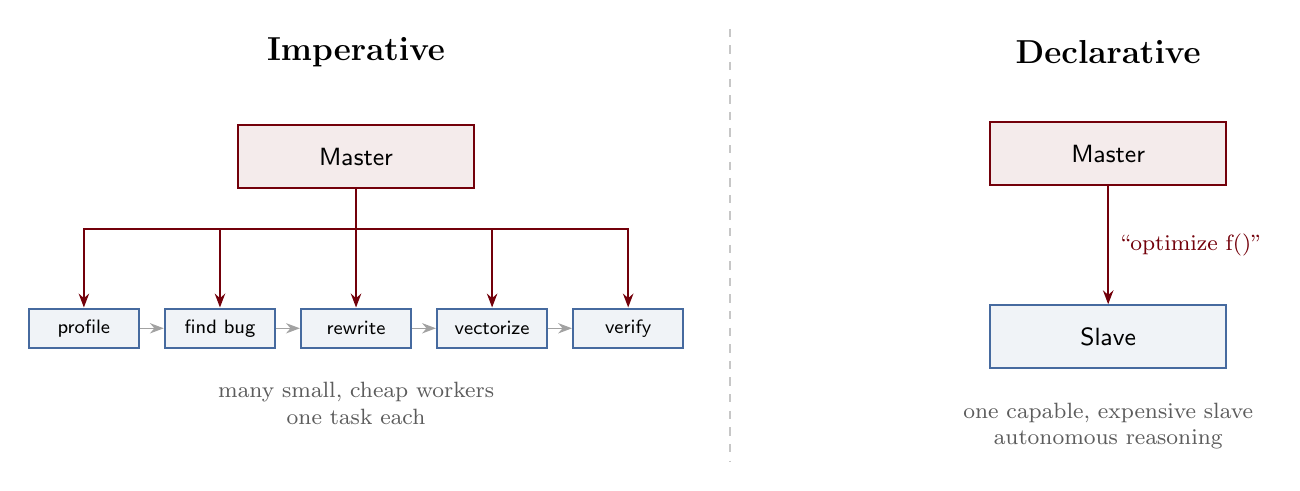
\begin{tikzpicture}[node distance=0.4cm and 0.8cm]

% === LEFT: Imperative ===
\node[font=\large\bfseries] (imp-title) {Imperative};

% Orchestrator
\node[agentbox=garnet, below=0.6cm of imp-title, minimum width=3cm] (imp-orch) {Master};

% Many small workers on same level, centered on orchestrator
\node[workerbox, below=1.5cm of imp-orch, minimum width=1.4cm, minimum height=0.5cm, font=\scriptsize\sffamily] (iw3) {rewrite};
\node[workerbox, left=0.3cm of iw3, minimum width=1.4cm, minimum height=0.5cm, font=\scriptsize\sffamily] (iw2) {find bug};
\node[workerbox, left=0.3cm of iw2, minimum width=1.4cm, minimum height=0.5cm, font=\scriptsize\sffamily] (iw1) {profile};
\node[workerbox, right=0.3cm of iw3, minimum width=1.4cm, minimum height=0.5cm, font=\scriptsize\sffamily] (iw4) {vectorize};
\node[workerbox, right=0.3cm of iw4, minimum width=1.4cm, minimum height=0.5cm, font=\scriptsize\sffamily] (iw5) {verify};

% 90-degree bend arrows
\draw[dataarrow=garnet] (imp-orch.south) -- ++(0,-0.5) -| (iw1.north);
\draw[dataarrow=garnet] (imp-orch.south) -- ++(0,-0.5) -| (iw2.north);
\draw[dataarrow=garnet] (imp-orch.south) -- ++(0,-0.5) -| (iw3.north);
\draw[dataarrow=garnet] (imp-orch.south) -- ++(0,-0.5) -| (iw4.north);
\draw[dataarrow=garnet] (imp-orch.south) -- ++(0,-0.5) -| (iw5.north);

% Small arrows between workers showing sequential dependency
\draw[dataarrow=bk50, thin] (iw1.east) -- (iw2.west);
\draw[dataarrow=bk50, thin] (iw2.east) -- (iw3.west);
\draw[dataarrow=bk50, thin] (iw3.east) -- (iw4.west);
\draw[dataarrow=bk50, thin] (iw4.east) -- (iw5.west);

% Label
\node[labelnode, below=0.3cm of iw3, font=\footnotesize, align=center] {many small, cheap workers\\one task each};

% === RIGHT: Declarative ===
\node[font=\large\bfseries, right=7cm of imp-title] (dec-title) {Declarative};

% Orchestrator (same size)
\node[agentbox=garnet, below=0.6cm of dec-title, minimum width=3cm] (dec-orch) {Master};

% One smart worker (same size as orchestrator)
\node[agentbox=atlantic, below=1.5cm of dec-orch, minimum width=3cm] (dw1) {Slave};

\draw[dataarrow=garnet] (dec-orch) -- (dw1)
  node[midway, right, font=\footnotesize] {``optimize f()''};

% Label
\node[labelnode, below=0.3cm of dw1, font=\footnotesize, align=center] {one capable, expensive slave\\autonomous reasoning};

% === Separator ===
\draw[dashed, bk30, thick] ($(imp-title.east)!0.5!(dec-title.west)$) ++(0,0.3) -- ++(0,-5.5);

\end{tikzpicture}
\caption{Imperative vs.\ declarative control models. With imperative control, the master decomposes work into micro-tasks and delegates each to a small, inexpensive slave. With declarative control, the master states the goal and a single capable slave reasons autonomously. The master's intelligence remains constant; what changes is the granularity of delegation.}
\label{fig:control_models}
\end{figure*}

Table~\ref{tab:control_comparison} summarizes the tradeoffs. Imperative control offers predictability at the cost of flexibility. Declarative control enables creative problem-solving but sacrifices determinism. Hybrid control, by allowing the master to tune the constraint set, provides a practical middle ground for most production agent systems.

\begin{table}[H]
\centering
\caption{Comparison of master control models.}
\label{tab:control_comparison}
\begin{tabularx}{\columnwidth}{lXXX}
\toprule
\textbf{Property} & \textbf{Imperative} & \textbf{Declarative} & \textbf{Hybrid} \\
\midrule
Intelligence location & Master & Slave & Shared \\
Message size & Large & Small & Medium \\
Worker autonomy & Low & High & Medium \\
Predictability & High & Low & Medium \\
Flexibility & Low & High & Medium \\
Best use case & Well-understood tasks with known solutions & Open-ended problems requiring creativity & Constrained optimization with clear requirements \\
\bottomrule
\end{tabularx}
\end{table}


% ── Part IV: Orchestrator Cycles (Sections 12-15) ─────────
%% Sections 12-15: Orchestration Patterns
%% Part of the Intro to Agents tutorial document

\section{The Orchestrator Cycle}\label{sec:orch_cycle}

Every orchestrator, regardless of its sophistication, executes some variant of a fundamental five-step loop: \textbf{Plan}, \textbf{Delegate}, \textbf{Wait}, \textbf{Collect}, and \textbf{Decide}. This cycle forms the operational heartbeat of master-worker architectures. The orchestrator begins by planning what work needs to be done, delegates tasks to subordinate agents, waits for those agents to complete their assignments, collects the results, and then decides what to do next — synthesize a final answer, iterate with refined tasks, or terminate.

The differences between orchestration strategies lie not in whether these steps occur, but in \emph{how} each step executes and whether the cycle repeats. A simple orchestrator may traverse the cycle exactly once, delegating all tasks upfront and terminating after collecting results. A sophisticated orchestrator may iterate through multiple cycles, refining its plan based on what previous workers discovered. A reactive orchestrator may skip explicit planning altogether, instead delegating minimal initial work and deciding on-the-fly how to respond to whatever comes back.

It is important to recognize that this five-step cycle is an \textbf{abstraction}, not a rigid implementation requirement. Real orchestrators may combine steps, reorder operations, or execute multiple steps concurrently. For example, an orchestrator might overlap the Wait and Delegate phases by launching new workers while waiting for earlier workers to complete, effectively pipelining the cycle. A reactive orchestrator might merge Plan and Decide into a single decision function that simultaneously evaluates results and determines next actions. Some implementations may delegate tasks to workers that themselves run mini-orchestration cycles, creating recursive delegation patterns that do not cleanly map to the linear five-step model. Despite these variations, the conceptual model remains useful: every orchestrator must identify work to be done, assign that work to agents, observe the outcomes, and determine whether to continue or terminate. The five-step abstraction provides a shared vocabulary for reasoning about orchestration strategies, even when the underlying implementations diverge from the idealized cycle.

Figure~\ref{fig:orch_single} illustrates the single-pass cycle: a straight line from Plan to Done with no feedback. Figure~\ref{fig:orch_iterative} shows the iterative variant, where a feedback loop from Decide back to Plan becomes the central mechanism for quality improvement and error recovery — the orchestrator explicitly routes control back to the planning phase for another round of delegation.

The sections that follow explore three fundamental orchestration patterns: single-pass orchestration (Section~\ref{sec:single_pass}), which traverses the cycle once and terminates; iterative orchestration (Section~\ref{sec:iterative}), which repeats the cycle until a quality threshold or iteration limit is reached; and reactive orchestration (Section~\ref{sec:reactive}), which abandons upfront planning in favor of event-driven adaptation. Each pattern represents a different trade-off between simplicity, robustness, and latency.

\begin{figure*}[t]
\centering
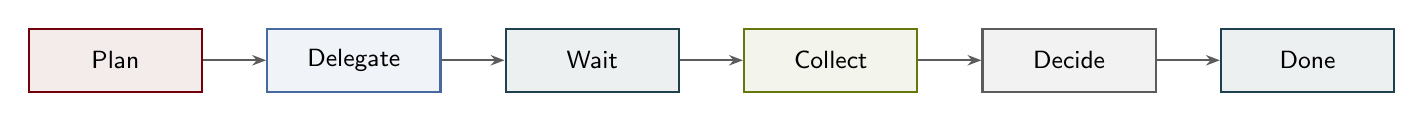
\begin{tikzpicture}[node distance=0.8cm and 0.8cm]
  \node[agentbox] (p1) {Plan};
  \node[agentbox=atlantic, right=of p1] (d1) {Delegate};
  \node[agentbox=congaree, right=of d1] (w1) {Wait};
  \node[agentbox=horseshoe, right=of w1] (c1) {Collect};
  \node[agentbox=bk70, right=of c1] (de1) {Decide};
  \node[agentbox=congaree, right=of de1] (done1) {Done};

  \draw[dataarrow] (p1) -- (d1);
  \draw[dataarrow] (d1) -- (w1);
  \draw[dataarrow] (w1) -- (c1);
  \draw[dataarrow] (c1) -- (de1);
  \draw[dataarrow] (de1) -- (done1);
\end{tikzpicture}
\caption{Single-pass orchestration cycle. The orchestrator traverses the five-step sequence Plan $\to$ Delegate $\to$ Wait $\to$ Collect $\to$ Decide exactly once, then terminates. There is no feedback loop and no opportunity to refine the plan based on worker results.}
\label{fig:orch_single}
\end{figure*}

\begin{figure*}[t]
\centering
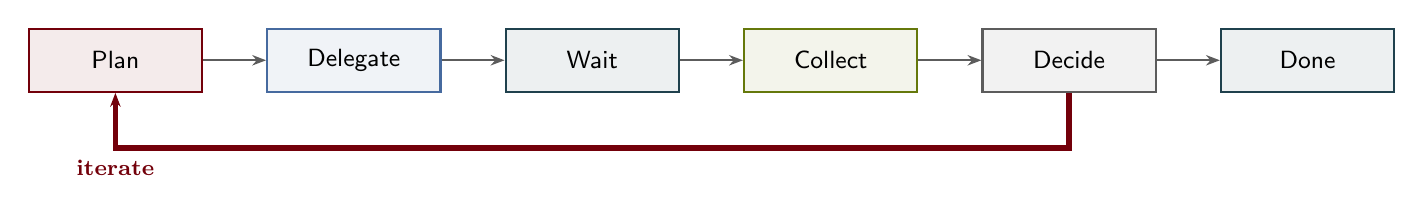
\begin{tikzpicture}[node distance=0.8cm and 0.8cm]
  \node[agentbox] (p2) {Plan};
  \node[agentbox=atlantic, right=of p2] (d2) {Delegate};
  \node[agentbox=congaree, right=of d2] (w2) {Wait};
  \node[agentbox=horseshoe, right=of w2] (c2) {Collect};
  \node[agentbox=bk70, right=of c2] (de2) {Decide};
  \node[agentbox=congaree, right=of de2] (done2) {Done};

  \draw[dataarrow] (p2) -- (d2);
  \draw[dataarrow] (d2) -- (w2);
  \draw[dataarrow] (w2) -- (c2);
  \draw[dataarrow] (c2) -- (de2);
  \draw[dataarrow] (de2) -- (done2);

  % Feedback loop: Decide back to Plan
  \draw[dataarrow, garnet, line width=2pt]
    (de2.south) -- ++(0,-0.7) -| (p2.south)
    node[pos=0.5, below, font=\footnotesize\bfseries] {iterate};
\end{tikzpicture}
\caption{Iterative orchestration cycle. The same five-step sequence, but with a feedback loop (bold arrow) from Decide back to Plan. After collecting results, the orchestrator evaluates quality and either terminates or iterates with refined tasks, enabling error recovery and progressive refinement.}
\label{fig:orch_iterative}
\end{figure*}

\section{Single-Pass Orchestration}\label{sec:single_pass}

The simplest orchestration model is the single-pass architecture: one traversal through the cycle, no iteration, no recovery. The orchestrator plans once, delegates all identified tasks to workers, waits for completion, collects results, synthesizes a final answer in the Decide phase, and terminates. This design prioritizes latency and simplicity. There are no feedback loops, no quality checks, and no opportunity to refine the plan based on what workers discover.

Single-pass orchestration works well when the problem is well-understood, the initial decomposition is correct, and workers reliably succeed. But these conditions rarely hold in practice. If the orchestrator misjudges the task breakdown — perhaps underestimating complexity or failing to anticipate dependencies — it has no recourse. If a worker fails due to an unavailable tool, an API timeout, or an unexpected data format, the master cannot retry, cannot delegate diagnostic work, and cannot adjust the plan. The orchestrator simply moves forward with whatever results it has.

This leads to a critical failure mode: \textbf{the orchestrator either gives up entirely or synthesizes a partial or hallucinated answer}. When faced with incomplete results, a single-pass orchestrator has two options. The first is to admit defeat, returning a message like ``I was unable to complete your task.'' The second, more insidious option is to produce an answer anyway, filling gaps with plausible-sounding but incorrect information synthesized from the fragments it managed to collect. Both outcomes are unacceptable for production systems, yet single-pass architectures are common in early-generation coding agents and task assistants.

The prevalence of single-pass orchestration in current coding agents explains many user frustrations with AI-assisted development tools. Consider a concrete example: a user asks an agent to refactor a Python module to use asynchronous I/O. The orchestrator decomposes this into three tasks: identify all synchronous I/O calls, update function signatures to use async/await, and update all call sites to await the new async functions. It delegates these tasks to three workers in parallel. The workers complete their assignments and return transformed code. The orchestrator collects the results, synthesizes them into a final patch, and presents it to the user. The user applies the patch, runs their test suite, and discovers that the application crashes on startup. The root cause: the refactoring also required updating configuration files that specify event loop policies, and the orchestrator never identified this as a required task. Because the orchestrator never considered configuration files in its initial decomposition, no worker was delegated to handle them, and the gap remained invisible until runtime. A single-pass orchestrator has no mechanism to detect such gaps — it cannot observe the test failure, cannot spawn a diagnostic worker to investigate, and cannot iterate to fill the missing piece. The result is broken code and a frustrated user who must either manually debug the issue or restart the entire interaction with more explicit instructions.

This failure mode is not an edge case; it is \textbf{the fundamental limitation of single-pass orchestration}. When the initial task decomposition is incomplete or incorrect, there is no recovery path. The orchestrator commits fully to its upfront plan, and any flaws in that plan propagate directly into the final output. Users experience this as the agent ``not understanding the full scope of the task,'' ``missing obvious dependencies,'' or ``breaking working code.'' From the orchestrator's perspective, however, it executed flawlessly: it planned, delegated, collected, and synthesized exactly as designed. The architecture itself provides no feedback loop through which the orchestrator might learn that its plan was insufficient.

The appeal of single-pass orchestration is its simplicity. There is no complex control flow, no iteration counters, no quality evaluation logic. The orchestrator is a straightforward pipeline: decompose, dispatch, wait, synthesize, done. But this simplicity comes at the cost of brittleness. Single-pass orchestrators fail silently, abandon tasks at the first obstacle, and provide no mechanism for the user or the system to understand why a failure occurred or how it might be remedied.

Figure~\ref{fig:orch_single} illustrates this flow. Once the orchestrator reaches the Decide phase, it either synthesizes a final answer and terminates successfully, or — because there is no path back to planning, no retry logic, and no recovery mechanism — it gives up entirely or produces a partial, potentially hallucinated result.

\section{Iterative Orchestration}\label{sec:iterative}

Iterative orchestration extends the base cycle by adding explicit feedback: after collecting results, the Decide phase evaluates whether the work is complete and of sufficient quality. If not, the orchestrator plans \emph{new} tasks informed by what it learned from previous workers, delegates those tasks, and repeats the cycle. This continues until one of three termination conditions is met: a \textbf{quality threshold} is reached, a \textbf{maximum iteration count} is exceeded, or the orchestrator determines that \textbf{no new tasks are necessary}.

The quality threshold termination condition requires the orchestrator to measure output quality against some objective or heuristic standard. In a coding agent, this might mean running a test suite and terminating when all tests pass, or invoking a static analyzer and iterating until all warnings are resolved. In a research assistant, it might mean evaluating a generated summary against a rubric of completeness and accuracy, using either a separate verification agent or a scoring function. The challenge is that many tasks lack clear quality metrics. How does an orchestrator measure whether a code refactoring is ``good enough''? One approach is to define proxy metrics: compilation succeeds, tests pass, code coverage remains stable, and static analysis reports no new issues. Another approach is to delegate the quality decision itself to a specialized verification agent that reviews the output and returns a binary approve/reject signal. Either way, the orchestrator must implement domain-specific evaluation logic in its Decide phase.

The maximum iteration count termination condition is a safety mechanism to prevent infinite loops. If the orchestrator cannot satisfy its quality threshold — perhaps the task is genuinely impossible, or the workers are repeatedly failing for systemic reasons — it must eventually give up rather than burning resources indefinitely. The iteration limit is typically a configuration parameter, tuned based on task complexity and acceptable latency. A simple task might cap at three iterations; a complex multi-step workflow might allow ten or twenty. When the limit is reached, the orchestrator either returns the best result achieved so far (a degraded success) or admits failure, depending on whether partial progress is useful to the user.

The no-new-tasks termination condition represents successful completion through exhaustion: the orchestrator has identified and executed all necessary work. This is distinct from reaching a quality threshold, because the orchestrator may complete all planned tasks and still fail to meet quality goals, triggering further iteration. Conversely, the orchestrator might reach the quality threshold before exhausting its task list, if earlier tasks turned out to be unnecessary or if workers exceeded expectations. The Decide phase must evaluate both dimensions — quality of output and completeness of task list — to determine whether to iterate or terminate.

Compared to single-pass orchestration, iterative orchestration is \textbf{strictly more capable} but incurs higher token and latency costs. An iterative orchestrator can recover from initial planning errors, adapt to unexpected worker results, and refine its approach through successive cycles. However, each cycle requires at least one additional LLM invocation in the Plan phase, plus the token costs of delegating new workers and evaluating their results. Latency multiplies linearly with iteration count, as each cycle must complete before the next begins. For tasks where a correct upfront plan is achievable, single-pass orchestration is more efficient. For tasks where the problem structure is uncertain or workers may fail unpredictably, the added cost of iteration is justified by the increased likelihood of successful completion.

The iterative model trades latency for quality and resilience. Where a single-pass orchestrator fails silently or gives up at the first obstacle, an iterative orchestrator can retry failed tasks with refined prompts, delegate diagnostic work to understand why a failure occurred, or spawn additional workers to fill gaps discovered during result synthesis. The orchestrator accumulates knowledge across iterations: each cycle refines the plan based on what previous workers discovered, what errors they encountered, and what intermediate results they produced.

Consider a concrete example: an orchestrator tasked with implementing a feature in a large codebase. In iteration one, it delegates a worker to locate the relevant module and another to identify dependencies. The first worker succeeds, but the second reports that the dependency graph is more complex than expected. In iteration two, the orchestrator spawns additional workers to trace transitive dependencies and verify API contracts. One of these workers discovers a breaking change in an upstream library. In iteration three, the orchestrator delegates a worker to implement a compatibility shim. Only after this third cycle does the Decide phase determine that all preconditions are satisfied and approve the final implementation.

This example illustrates the core advantage of iterative orchestration: \textbf{it transforms brittle failure into adaptive problem-solving}. The orchestrator does not need a perfect plan upfront; it can discover the true structure of the problem through successive refinement. Failed workers provide information — error messages, partial results, diagnostic traces — that the orchestrator uses to improve its next attempt.

However, iteration introduces new challenges. The orchestrator must maintain state across cycles, tracking which tasks have been attempted, which have succeeded, and which need refinement. It must implement a quality evaluation function in the Decide phase, which may require domain-specific heuristics or external verification tools. And it must guard against infinite loops, implementing termination logic that balances thoroughness with resource constraints.

Figure~\ref{fig:orch_iterative} shows the iterative cycle with the feedback loop from Decide to Plan rendered as a bold arrow labeled ``iterate.'' This loop is the defining characteristic of iterative orchestration. The orchestrator also includes an exit path labeled ``done,'' taken when a termination condition is met. The challenge in implementing iterative orchestration lies in deciding when to iterate and when to exit — a decision that depends on the task domain, the quality of intermediate results, and the cost of additional cycles.

\section{Reactive Orchestration}\label{sec:reactive}

Reactive orchestration abandons upfront planning altogether. Instead of decomposing the entire task before delegating any work, a reactive orchestrator starts with a minimal initial action — perhaps a single diagnostic query or a broad exploratory task — and then reacts to whatever comes back. If a worker succeeds, the orchestrator decides whether to continue along the same path or terminate. If a worker returns an error, the orchestrator spawns a diagnostic worker to investigate. If a worker discovers something unexpected — a missing file, an API incompatibility, a hidden dependency — the orchestrator adjusts its approach, delegating new tasks to handle the surprise.

This is \textbf{event-driven} orchestration, not plan-driven. The orchestrator maintains minimal state and makes local decisions based on the most recent worker output. It does not attempt to construct a complete task graph upfront; instead, it builds the graph incrementally, one node at a time, guided by the results it observes. This makes reactive orchestration particularly well-suited for exploratory tasks where the problem space is poorly understood: debugging, codebase exploration, open-ended research, or adversarial testing.

Consider debugging a test failure in an unfamiliar codebase. A plan-driven orchestrator would attempt to decompose the problem upfront: read the test file, identify the failing assertion, trace dependencies, inspect relevant modules, and so on. But this decomposition requires knowledge the orchestrator does not yet have — which modules are relevant? What dependencies matter? A reactive orchestrator, by contrast, begins with a single action: run the test and capture the failure output. It then reacts to that output. If the failure is a missing import, it delegates a worker to locate the missing module. If the failure is an assertion mismatch, it delegates a worker to inspect the function under test. Each worker output informs the next delegation.

The advantage of reactive orchestration is its \textbf{adaptability}. The orchestrator does not commit to a fixed plan; it responds dynamically to the structure of the problem as it emerges. This reduces upfront planning overhead and avoids the pitfall of executing a plan that turns out to be inappropriate. The disadvantage is increased latency: each delegation requires a round-trip to a worker, and the orchestrator cannot parallelize tasks that might have been identified through upfront planning.

Reactive orchestration also places greater demands on the orchestrator's decision-making. Without a plan to guide it, the orchestrator must decide at each step whether it has enough information to proceed, whether it needs to investigate further, or whether it should terminate. These decisions require either sophisticated heuristics or a powerful decision model — often the orchestrator itself is a large language model capable of reasoning about partial information and uncertain outcomes.

Figure~\ref{fig:reactive} illustrates the reactive orchestration pattern. A central orchestrator delegates tasks to workers and receives three types of responses: success (the worker completed its task, and the orchestrator can continue or terminate), error (the worker failed, triggering delegation to a diagnostic agent), and unexpected (the worker discovered something that requires replanning). These three branches represent the core reactive logic: \textbf{adapt to what you learn, do not commit to what you assumed}.

\begin{figure*}[t]
\centering
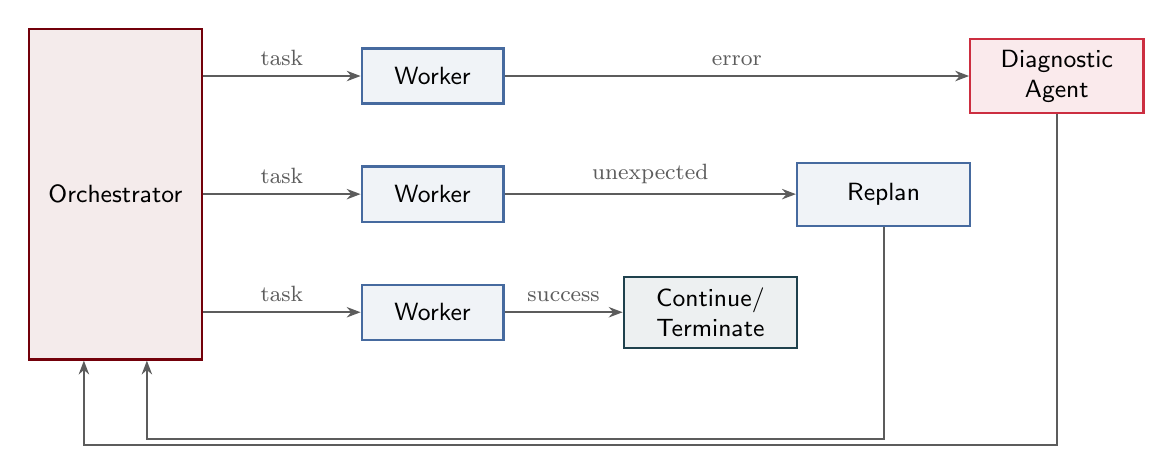
\begin{tikzpicture}[node distance=0.8cm and 1.0cm]

  % Orchestrator on the left, tall to span all three rows
  \node[agentbox, minimum height=4.2cm, minimum width=2.2cm] (orch) {Orchestrator};

  % Row 1: Error / Diagnostic (top)
  \node[workerbox, right=2.0cm of orch, yshift=1.5cm] (w2) {Worker};
  \node[failbox, right=5.9cm of w2, minimum width=2.2cm] (diag) {Diagnostic\\Agent};

  \draw[dataarrow] (orch.east |- w2) -- node[above,font=\footnotesize] {task} (w2);
  \draw[dataarrow] (w2) -- node[above,font=\footnotesize] {error} (diag);
  % Diagnostic loops back: go down under everything, then left to orchestrator bottom
  \draw[dataarrow] (diag.south) -- ++(0,-4.2) -| ([xshift=-0.4cm]orch.south);

  % Row 2: Unexpected / Replan (middle)
  \node[workerbox, right=2.0cm of orch] (w3) {Worker};
  \node[agentbox=atlantic, right=3.7cm of w3, minimum width=2.2cm] (replan) {Replan};

  \draw[dataarrow] (orch.east |- w3) -- node[above,font=\footnotesize] {task} (w3);
  \draw[dataarrow] (w3) -- node[above,font=\footnotesize] {unexpected} (replan);
  % Replan loops back: go down under everything, then left to orchestrator bottom
  \draw[dataarrow] (replan.south) -- ++(0,-2.7) -| ([xshift=0.4cm]orch.south);

  % Row 3: Success / Continue (bottom)
  \node[workerbox, right=2.0cm of orch, yshift=-1.5cm] (w1) {Worker};
  \node[agentbox=congaree, right=1.5cm of w1, minimum width=2.2cm] (cont) {Continue/\\Terminate};

  \draw[dataarrow] (orch.east |- w1) -- node[above,font=\footnotesize] {task} (w1);
  \draw[dataarrow] (w1) -- node[above,font=\footnotesize] {success} (cont);

\end{tikzpicture}
\caption{Reactive orchestration pattern. The orchestrator delegates tasks and reacts to three types of outcomes: unexpected (top row --- worker discovers something surprising, triggering replanning and a new orchestration cycle), error (middle row --- worker fails, diagnostic agent investigates and feeds back to the orchestrator), and success (bottom row --- worker completes, orchestrator continues or terminates).}
\label{fig:reactive}
\end{figure*}


% ── Part V: Topology & Patterns (Sections 16-20) ──────────
%% Sections 16-20: Topology and Orchestration Patterns
%% Part of Intro_to_Agents article
%% Author: J.C. Vaught

\section{Serial Agent Chains}\label{sec:serial}

In a serial agent chain, workers execute sequentially, forming a pipeline topology. The output of Worker A becomes the input to Worker B, which feeds Worker C, and so on. The master orchestrator coordinates handoffs between stages, ensuring each worker receives the correct input at the appropriate time.

This topology maps naturally onto transformation chains, where data must pass through multiple processing stages in a fixed order. For example, a document processing pipeline might parse raw text, analyze its structure, and format the output. Each stage depends on the previous stage's output, making parallelization impossible. Similarly, refinement chains implement sequential improvement: an initial draft is generated, reviewed for quality, and then revised based on feedback.

The serial topology offers predictability and simplicity. Dependencies are explicit and linear. Debugging is straightforward because you can inspect the data flowing between each stage. The primary limitation is latency: total execution time equals the sum of all stage durations, with no opportunity for parallel speedup.

\begin{figure*}[t]
\centering
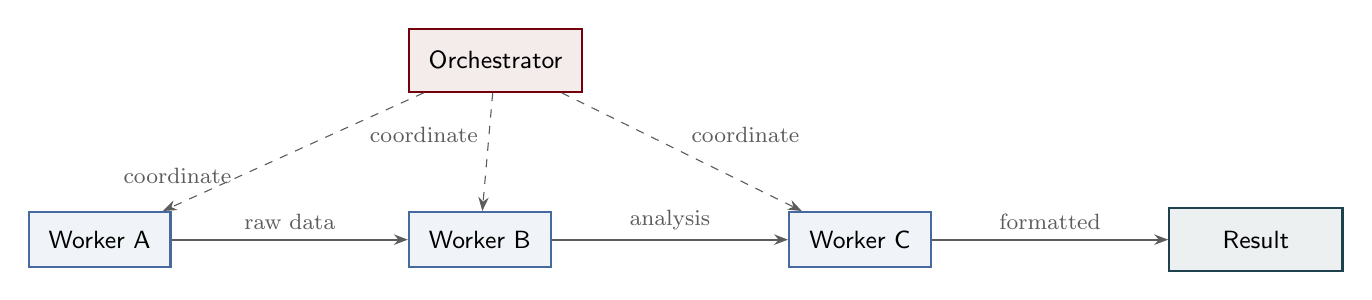
\begin{tikzpicture}[node distance=2.5cm and 3cm]
  % Orchestrator at top
  \node[agentbox=garnet] (orch) {Orchestrator};

  % Pipeline workers
  \node[workerbox, below left=1.5cm and 3cm of orch] (wa) {Worker A};
  \node[workerbox, right=of wa] (wb) {Worker B};
  \node[workerbox, right=of wb] (wc) {Worker C};
  \node[agentbox=congaree, right=of wc] (result) {Result};

  % Pipeline flow
  \draw[dataarrow] (wa) -- node[above] {\footnotesize raw data} (wb);
  \draw[dataarrow] (wb) -- node[above] {\footnotesize analysis} (wc);
  \draw[dataarrow] (wc) -- node[above] {\footnotesize formatted} (result);

  % Coordination from orchestrator
  \draw[dataarrow, dashed, thin] (orch) -- node[left, pos=0.7] {\footnotesize coordinate} (wa);
  \draw[dataarrow, dashed, thin] (orch) -- node[above left, pos=0.5] {\footnotesize coordinate} (wb);
  \draw[dataarrow, dashed, thin] (orch) -- node[above right, pos=0.5] {\footnotesize coordinate} (wc);
\end{tikzpicture}
\caption{Serial agent chain with orchestrated handoffs. Each worker processes its input and passes results to the next stage.}
\label{fig:serial_chain}
\end{figure*}

Figure~\ref{fig:serial_chain} illustrates the serial topology. The orchestrator coordinates the pipeline but does not participate in data transformation. Workers operate independently once launched, with coordination limited to handoff timing and error handling.

\section{Parallel Agent Execution}\label{sec:parallel_agents}

Parallel agent execution enables workers to operate simultaneously on independent tasks. The orchestrator fans out work and collects results. Unlike serial chains, parallel execution offers the potential for significant speedup when tasks are independent and workers have sufficient computational resources.

The key challenge in parallel execution is synchronization: when should the orchestrator proceed with the results it has received? Three barrier types govern this decision, each suited to different requirements.

A \textbf{full barrier} waits for all workers to complete before proceeding. This is required when every result is necessary for correctness. For example, when aggregating statistics across multiple data partitions, missing even one partition would corrupt the final result. Full barriers maximize correctness at the cost of latency: the slowest worker determines total execution time.

A \textbf{partial barrier} or k-of-n barrier proceeds when k workers finish, where k < n. This pattern supports consensus mechanisms (majority vote requires $k > n/2$) and redundant task execution (take the first k results and discard the rest). Partial barriers reduce sensitivity to slow workers but require careful design to ensure that proceeding with incomplete results does not violate correctness requirements.

A \textbf{timeout barrier} waits up to t seconds, then proceeds with whatever results are available. This implements best-effort execution: the system prioritizes responsiveness over completeness. Timeout barriers are appropriate when partial results have value and when strict deadlines matter more than exhaustive coverage. The orchestrator must handle missing results gracefully, either by synthesizing incomplete data or by flagging gaps in coverage.

\begin{figure*}[t]
\centering
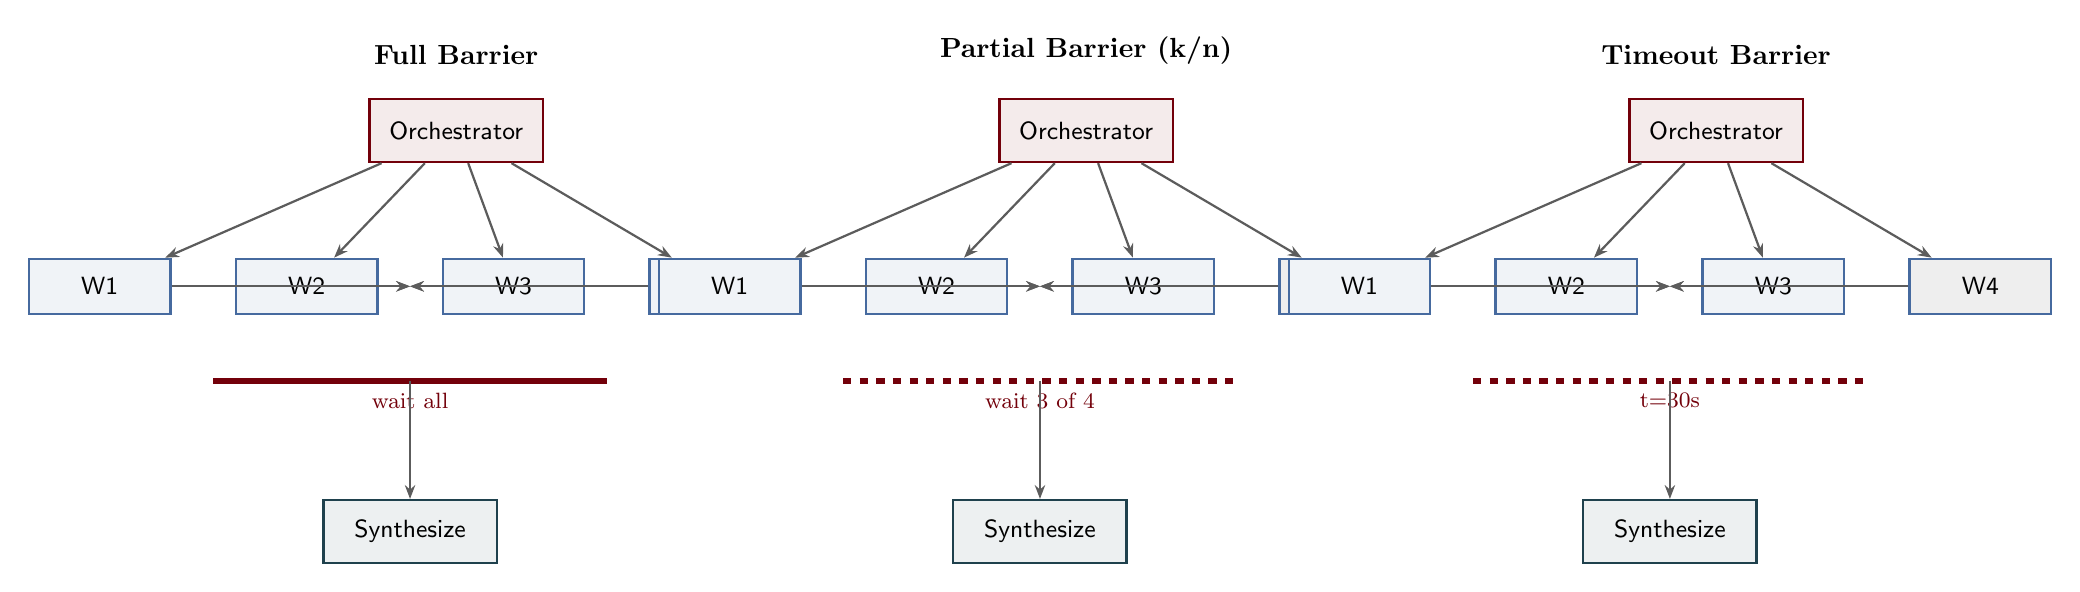
\begin{tikzpicture}[node distance=1.2cm and 1.5cm]
  % Full Barrier
  \node[agentbox=garnet] (orch1) {Orchestrator};
  \node[workerbox, below left=of orch1, xshift=-1cm] (w11) {W1};
  \node[workerbox, right=0.8cm of w11] (w12) {W2};
  \node[workerbox, right=0.8cm of w12] (w13) {W3};
  \node[workerbox, right=0.8cm of w13] (w14) {W4};

  \coordinate (barrier1) at ($(w11)!0.5!(w14) + (0,-1.2)$);
  \draw[line width=2pt, garnet] ($(barrier1) + (-2.5,0)$) -- node[below, pos=0.5] {\footnotesize wait all} ($(barrier1) + (2.5,0)$);

  \node[agentbox=congaree, below=1.5cm of barrier1] (syn1) {Synthesize};

  \foreach \w in {w11,w12,w13,w14} {
    \draw[dataarrow] (orch1) -- (\w);
    \draw[dataarrow] (\w) -- (barrier1 |- \w);
  }
  \draw[dataarrow] (barrier1) -- (syn1);

  \node[above=0.3cm of orch1, font=\bfseries] {Full Barrier};

  % Partial Barrier
  \begin{scope}[xshift=8cm]
    \node[agentbox=garnet] (orch2) {Orchestrator};
    \node[workerbox, below left=of orch2, xshift=-1cm] (w21) {W1};
    \node[workerbox, right=0.8cm of w21] (w22) {W2};
    \node[workerbox, right=0.8cm of w22] (w23) {W3};
    \node[workerbox, right=0.8cm of w23, fill=bk30!30] (w24) {W4};

    \coordinate (barrier2) at ($(w21)!0.5!(w24) + (0,-1.2)$);
    \draw[line width=2pt, garnet, dashed] ($(barrier2) + (-2.5,0)$) -- node[below, pos=0.5] {\footnotesize wait 3 of 4} ($(barrier2) + (2.5,0)$);

    \node[agentbox=congaree, below=1.5cm of barrier2] (syn2) {Synthesize};

    \foreach \w in {w21,w22,w23,w24} {
      \draw[dataarrow] (orch2) -- (\w);
      \draw[dataarrow] (\w) -- (barrier2 |- \w);
    }
    \draw[dataarrow] (barrier2) -- (syn2);

    \node[above=0.3cm of orch2, font=\bfseries] {Partial Barrier (k/n)};
  \end{scope}

  % Timeout Barrier
  \begin{scope}[xshift=16cm]
    \node[agentbox=garnet] (orch3) {Orchestrator};
    \node[workerbox, below left=of orch3, xshift=-1cm] (w31) {W1};
    \node[workerbox, right=0.8cm of w31] (w32) {W2};
    \node[workerbox, right=0.8cm of w32] (w33) {W3};
    \node[workerbox, right=0.8cm of w33, fill=bk30!30] (w34) {W4};

    \coordinate (barrier3) at ($(w31)!0.5!(w34) + (0,-1.2)$);
    \draw[line width=2pt, garnet, dashed] ($(barrier3) + (-2.5,0)$) -- node[below, pos=0.5] {\footnotesize t=30s} ($(barrier3) + (2.5,0)$);

    \node[agentbox=congaree, below=1.5cm of barrier3] (syn3) {Synthesize};

    \foreach \w in {w31,w32,w33,w34} {
      \draw[dataarrow] (orch3) -- (\w);
      \draw[dataarrow] (\w) -- (barrier3 |- \w);
    }
    \draw[dataarrow] (barrier3) -- (syn3);

    \node[above=0.3cm of orch3, font=\bfseries] {Timeout Barrier};
  \end{scope}
\end{tikzpicture}
\caption{Three barrier types for parallel execution. Full barriers wait for all workers. Partial barriers proceed when k workers finish. Timeout barriers enforce deadlines.}
\label{fig:parallel_exec}
\end{figure*}

Figure~\ref{fig:parallel_exec} compares the three barrier types. Grayed workers in the partial and timeout variants indicate workers whose results are not required for the orchestrator to proceed. The choice of barrier depends on the task's tolerance for incomplete results and its latency requirements.

\section{Tree-Structured Agent Hierarchies}\label{sec:tree}

Tree-structured hierarchies extend the master-worker pattern with intermediate delegation layers. A root master delegates to lead agents, who in turn delegate to specialist workers. This topology is about the shape of delegation, not about formal layering or rigid role definitions.

Information flows bidirectionally in a tree hierarchy. Tasks and context flow downward via solid edges: the root provides high-level goals to leads, who decompose them into subtasks for specialists. Results and status flow upward via dashed edges: specialists report to leads, who synthesize and report to the root. Each node acts as both a worker (for its parent) and a master (for its children).

\begin{figure*}[t]
\centering
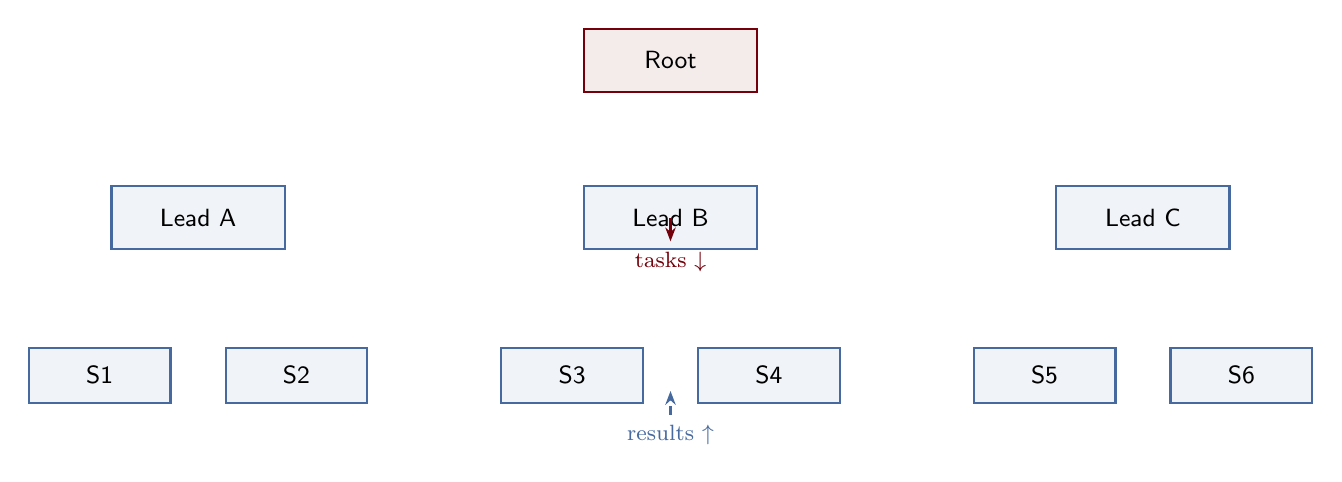
\begin{tikzpicture}[
  level 1/.style={sibling distance=6cm, level distance=2cm},
  level 2/.style={sibling distance=2.5cm, level distance=2cm},
  edge from parent/.style={dataarrow=garnet},
  edge from parent path={(\tikzparentnode.south) -- (\tikzchildnode.north)}
]
  \node[agentbox=garnet] {Root}
    child {
      node[agentbox=atlantic] {Lead A}
      child { node[workerbox] {S1} }
      child { node[workerbox] {S2} }
    }
    child {
      node[agentbox=atlantic] {Lead B}
      child { node[workerbox] {S3} }
      child { node[workerbox] {S4} }
    }
    child {
      node[agentbox=atlantic] {Lead C}
      child { node[workerbox] {S5} }
      child { node[workerbox] {S6} }
    };

  % Add upward dashed arrows (results flow)
  \draw[dataarrow=atlantic, dashed] (0,-4.5) -- ++(0,0.3) node[pos=0, below] {\footnotesize results $\uparrow$};
  \draw[dataarrow=garnet] (0,-2) -- ++(0,-0.3) node[pos=1, below] {\footnotesize tasks $\downarrow$};

  % Side labels removed (already shown on arrows above)
\end{tikzpicture}
\caption{Tree-structured agent hierarchy with three levels. Tasks flow down (solid arrows), results flow up (dashed arrows).}
\label{fig:tree_hierarchy}
\end{figure*}

Tree hierarchies enable delegation at scale, but depth is limited by token costs. Each level multiplies total token consumption: if the root's prompt is 1000 tokens and each lead receives a similar context, and each specialist likewise, the total context across all agents can reach tens of thousands of tokens. Practical systems rarely exceed three levels due to these costs and the coordination overhead of deep hierarchies.

Figure~\ref{fig:tree_hierarchy} shows a three-level tree. The root delegates to three leads, each managing two specialists. Solid edges represent task delegation; dashed edges represent result aggregation. The root never communicates directly with specialists; all communication is mediated by the leads.

\section{Unidirectional vs.\ Bidirectional Communication}\label{sec:uni_bi}

Communication between master and worker can be unidirectional or bidirectional. The choice affects protocol complexity, adaptability, and predictability.

In \textbf{unidirectional communication}, the master sends a task and the worker returns a result. No mid-task communication occurs. The worker cannot ask for clarification, request additional context, or negotiate scope. It must work with what it was given. This simplicity offers isolation and predictability: each worker operates independently, and the master's responsibilities are limited to task assignment and result collection.

Unidirectional communication is appropriate when tasks are well-specified and workers have sufficient context to operate autonomously. The cost of this simplicity is rigidity: if the worker encounters ambiguity or missing information, it must make assumptions or fail. The master has no opportunity to intervene mid-task.

In \textbf{bidirectional communication}, the worker can interrupt the master to ask questions, request clarification, or negotiate scope changes. This adaptability enables workers to handle underspecified tasks and to refine their approach based on runtime discoveries. The master must handle interrupts, which complicates the orchestration protocol. Bidirectional communication increases coupling: the master and worker must agree on an interrupt protocol, and the master's availability becomes a bottleneck.

\begin{figure*}[t]
\centering
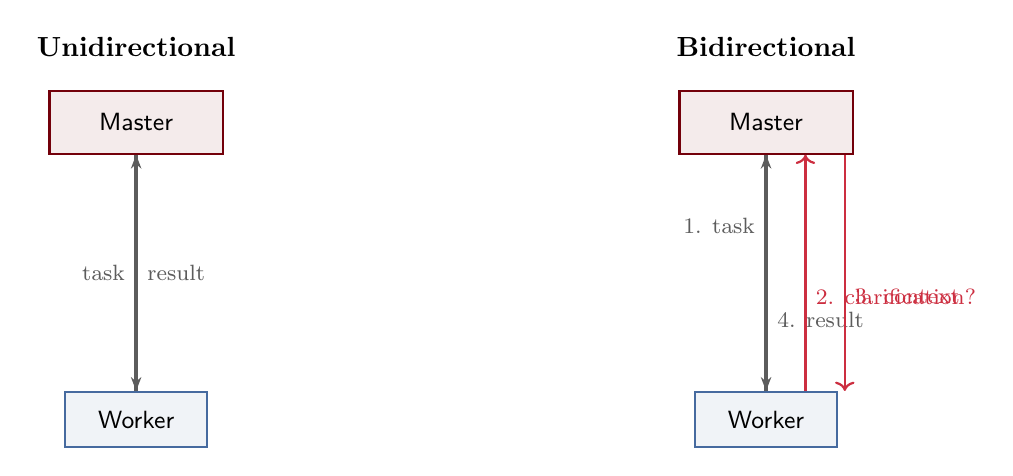
\begin{tikzpicture}[node distance=3cm and 6cm]
  % Unidirectional
  \node[agentbox=garnet] (m1) {Master};
  \node[workerbox, below=of m1] (w1) {Worker};

  \draw[dataarrow, line width=1.5pt] (m1) -- node[left] {\footnotesize task} (w1);
  \draw[dataarrow, dashed, line width=1.5pt] (w1) -- node[right] {\footnotesize result} (m1);

  \node[above=0.3cm of m1, font=\bfseries] {Unidirectional};

  % Bidirectional
  \begin{scope}[xshift=8cm]
    \node[agentbox=garnet] (m2) {Master};
    \node[workerbox, below=of m2] (w2) {Worker};

    \draw[dataarrow, line width=1.5pt] (m2) -- node[left, pos=0.3] {\footnotesize 1. task} (w2);
    \draw[dataarrow, dashed, line width=1.5pt] (w2) -- node[right, pos=0.3] {\footnotesize 4. result} (m2);

    % Mid-task communication
    \draw[dataarrow=rose, ->] ($(w2.north) + (0.5,0)$) -- node[right, pos=0.4] {\footnotesize\color{rose} 2. clarification?} ($(m2.south) + (0.5,0)$);
    \draw[dataarrow=rose, ->] ($(m2.south) + (1.0,0)$) -- node[right, pos=0.6] {\footnotesize\color{rose} 3. context} ($(w2.north) + (1.0,0)$);

    \node[above=0.3cm of m2, font=\bfseries] {Bidirectional};
  \end{scope}
\end{tikzpicture}
\caption{Unidirectional communication (left) vs.\ bidirectional communication (right). Bidirectional workers can request clarification mid-task.}
\label{fig:uni_vs_bi}
\end{figure*}

Figure~\ref{fig:uni_vs_bi} contrasts the two models. The unidirectional case shows a clean request-response cycle. The bidirectional case adds mid-task clarification (step 2) and additional context (step 3), shown in a distinct color to emphasize the interrupt protocol. Sequence numbers indicate the temporal ordering of messages.

\section{Canonical Orchestration Patterns}\label{sec:canonical}

The building blocks introduced in previous sections combine to form four canonical orchestration patterns. Each pattern represents a distinct solution to a recurring coordination problem.

The \textbf{pipeline} pattern combines serial topology, single-pass orchestration, and unidirectional communication. It implements transformation chains where data flows through sequential stages. Each stage performs a well-defined transformation and passes results forward. The pattern is simple and predictable but offers no parallelism.

The \textbf{fan-out/fan-in} pattern combines parallel topology, single-pass orchestration, and unidirectional communication. The orchestrator fans out independent subtasks to multiple workers and synthesizes their results. This pattern exploits task parallelism for speedup but requires that subtasks be independent.

The \textbf{master-worker pool} pattern combines parallel topology, iterative orchestration, and unidirectional communication. The master maintains a queue of tasks and assigns them to workers as they become available. Workers execute tasks independently and return results. The master continues until the queue is empty. This pattern efficiently handles batch processing and load balancing.

The \textbf{feedback loop} pattern combines serial topology, iterative orchestration, and bidirectional communication. The planner generates a plan, the executor attempts it, and the executor reports results back to the planner for refinement. This pattern enables iterative improvement and adaptive planning but incurs higher coordination overhead.

\begin{figure*}[t]
\centering
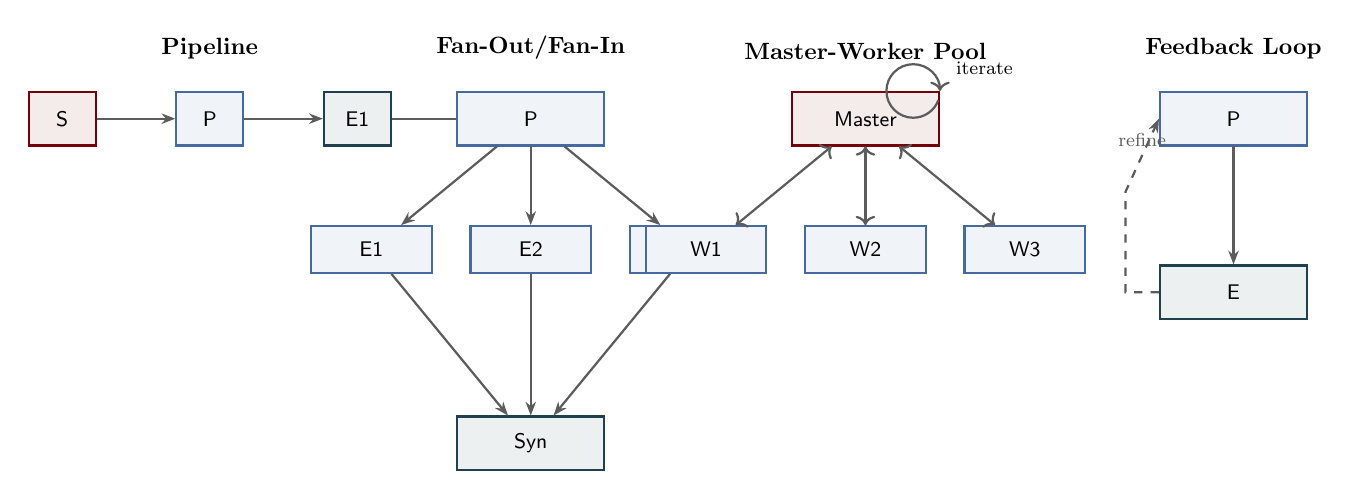
\begin{tikzpicture}[node distance=1.2cm and 1.5cm, scale=0.85, every node/.style={scale=0.85}]
  % Pipeline
  \node[agentbox=garnet, minimum width=1cm] (p1) {S};
  \node[agentbox=atlantic, right=1cm of p1, minimum width=1cm] (p2) {P};
  \node[agentbox=congaree, right=1cm of p2, minimum width=1cm] (p3) {E1};
  \node[agentbox=horseshoe, right=1cm of p3, minimum width=1cm] (p4) {E2};

  \draw[dataarrow] (p1) -- (p2);
  \draw[dataarrow] (p2) -- (p3);
  \draw[dataarrow] (p3) -- (p4);

  \node[above=0.3cm of p2, font=\bfseries] {Pipeline};

  % Fan-Out/Fan-In
  \begin{scope}[xshift=7cm]
    \node[agentbox=atlantic] (fo1) {P};
    \node[workerbox, below left=1cm and 0.3cm of fo1] (fo2) {E1};
    \node[workerbox, below=1cm of fo1] (fo3) {E2};
    \node[workerbox, below right=1cm and 0.3cm of fo1] (fo4) {E3};
    \node[agentbox=congaree, below=1.8cm of fo3] (fo5) {Syn};

    \foreach \w in {fo2,fo3,fo4} {
      \draw[dataarrow] (fo1) -- (\w);
      \draw[dataarrow] (\w) -- (fo5);
    }

    \node[above=0.3cm of fo1, font=\bfseries] {Fan-Out/Fan-In};
  \end{scope}

  % Master-Worker Pool
  \begin{scope}[xshift=12cm]
    \node[agentbox=garnet] (mw1) {Master};
    \node[workerbox, below left=1cm and 0.3cm of mw1] (mw2) {W1};
    \node[workerbox, below=1cm of mw1] (mw3) {W2};
    \node[workerbox, below right=1cm and 0.3cm of mw1] (mw4) {W3};

    \foreach \w in {mw2,mw3,mw4} {
      \draw[dataarrow, <->] (mw1) -- (\w);
    }

    \draw[dataarrow, <-] (mw1.north east) arc[start angle=0, end angle=340, radius=0.4cm];
    \node[above right=0.1cm and 0.1cm of mw1, font=\footnotesize] {iterate};

    \node[above=0.3cm of mw1, font=\bfseries] {Master-Worker Pool};
  \end{scope}

  % Feedback Loop
  \begin{scope}[xshift=17.5cm]
    \node[agentbox=atlantic] (fb1) {P};
    \node[agentbox=congaree, below=1.5cm of fb1] (fb2) {E};

    \draw[dataarrow] (fb1) -- (fb2);
    \draw[dataarrow, dashed] (fb2.west) -- ++(-0.5,0) -- ++(0,1.5) -- node[above, pos=0.5] {\footnotesize refine} (fb1.west);

    \node[above=0.3cm of fb1, font=\bfseries] {Feedback Loop};
  \end{scope}
\end{tikzpicture}
\caption{Four canonical orchestration patterns. Each combines topology, orchestration mode, and communication direction in a distinct way.}
\label{fig:canonical_summary}
\end{figure*}

Figure~\ref{fig:canonical_summary} visualizes these four patterns. Each diagram uses consistent node sizes and color coding to emphasize structural differences. Table~\ref{tab:pattern_decision} maps each pattern onto its constituent building blocks and identifies its primary use case.

\begin{table}[t]
\centering
\caption{Canonical orchestration patterns and their building blocks.}
\label{tab:pattern_decision}
\begin{tabularx}{\columnwidth}{lXlll}
\toprule
\textbf{Pattern} & \textbf{Topology} & \textbf{Orchestration} & \textbf{Direction} & \textbf{Best For} \\
\midrule
Pipeline & Serial & Single-pass & Unidirectional & Transformation chains \\
Fan-Out/Fan-In & Parallel & Single-pass & Unidirectional & Independent subtasks \\
Master-Worker Pool & Parallel & Iterative & Unidirectional & Batch processing \\
Feedback Loop & Serial & Iterative & Bidirectional & Iterative refinement \\
\bottomrule
\end{tabularx}
\end{table}

These patterns are not mutually exclusive. Real systems often combine multiple patterns within a single architecture, nesting fan-out within a pipeline stage or embedding a feedback loop inside a worker pool. The value of canonical patterns lies in their composability: once you understand the primitives, you can combine them to build arbitrarily complex orchestration logic.


% ── Part VI: Multi-Layered (Sections 21-25) ───────────────
%% Sections 21-25: Multi-Layered Agent Architectures
%% This file is meant to be \input into a two-column LaTeX article

\section{Why Multi-Layered Architectures?}\label{sec:why_layers}

A flat master model—one master managing everything—creates a bottleneck. As task complexity grows, the master's context fills with operational details: which files were changed, what errors occurred, what each slave reported. The master loses sight of the big picture. Consider an analogy: a CEO who personally writes deployment scripts has no time left for strategy. The fundamental problem is one of cognitive load. A single agent cannot simultaneously hold strategic vision, tactical planning, and execution details within a finite context window.

Layering separates concerns. Strategic decisions occur at the top layer, where the agent reasons about goals, constraints, and success criteria. Tactical planning happens in the middle, where goals decompose into concrete task graphs with dependencies. Execution happens at the bottom, where specialized slaves perform individual operations and report results. Each layer filters and abstracts information before passing it upward or downward. This separation is what allows multi-agent systems to scale beyond the limitations of a single context window.

\begin{figure*}[t]
\centering
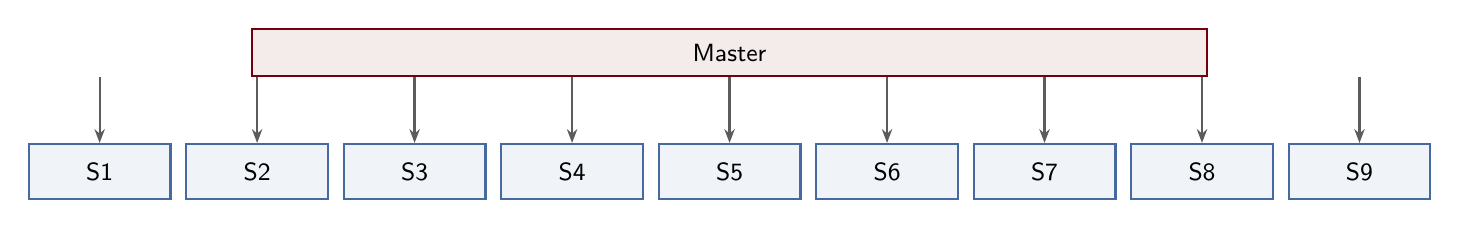
\begin{tikzpicture}[node distance=0.8cm and 0.8cm]
  % Master - text width bar
  \node[agentbox=garnet, minimum width=\textwidth, minimum height=0.6cm] (master) {Master};

  % 9 slaves in one row, equally spaced across text width
  \node[workerbox] at ([yshift=-1.2cm, xshift=-8cm]master.south) (w1) {S1};
  \node[workerbox] at ([yshift=-1.2cm, xshift=-6cm]master.south) (w2) {S2};
  \node[workerbox] at ([yshift=-1.2cm, xshift=-4cm]master.south) (w3) {S3};
  \node[workerbox] at ([yshift=-1.2cm, xshift=-2cm]master.south) (w4) {S4};
  \node[workerbox] at ([yshift=-1.2cm]master.south) (w5) {S5};
  \node[workerbox] at ([yshift=-1.2cm, xshift=2cm]master.south) (w6) {S6};
  \node[workerbox] at ([yshift=-1.2cm, xshift=4cm]master.south) (w7) {S7};
  \node[workerbox] at ([yshift=-1.2cm, xshift=6cm]master.south) (w8) {S8};
  \node[workerbox] at ([yshift=-1.2cm, xshift=8cm]master.south) (w9) {S9};

  % Arrows from master to each slave
  \foreach \w in {w1,w2,w3,w4,w5,w6,w7,w8,w9} {
    \draw[dataarrow] (master.south -| \w) -- (\w);
  }
\end{tikzpicture}
\caption{Flat architecture: a single master coordinates directly with every slave. The master must hold both strategic and tactical context ($\sim$80K tokens), while each slave operates with a smaller, task-specific context ($\sim$30K tokens). As the number of slaves grows, the master's context fills with operational details, leading to context overload.}
\label{fig:flat_architecture}
\end{figure*}

\begin{figure*}[t]
\centering
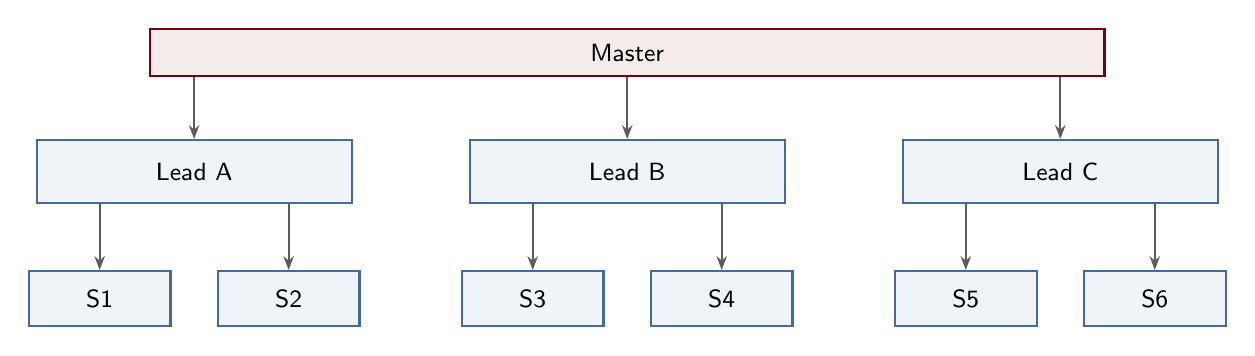
\begin{tikzpicture}[node distance=0.8cm and 0.8cm]
  % Root Master - text width bar
  \node[agentbox=garnet, minimum width=\textwidth, minimum height=0.6cm] (root) {Master};

  % Lead row (intermediate masters) - centered
  \node[agentbox=atlantic, minimum width=4cm] at ([yshift=-1.2cm, xshift=-5.5cm]root.south) (leadA) {Lead A};
  \node[agentbox=atlantic, minimum width=4cm] at ([yshift=-1.2cm]root.south) (leadB) {Lead B};
  \node[agentbox=atlantic, minimum width=4cm] at ([yshift=-1.2cm, xshift=5.5cm]root.south) (leadC) {Lead C};

  % Arrows from root to leads
  \draw[dataarrow] (root.south -| leadA) -- (leadA);
  \draw[dataarrow] (root.south -| leadB) -- (leadB);
  \draw[dataarrow] (root.south -| leadC) -- (leadC);

  % Slaves under Lead A
  \node[workerbox] at ([yshift=-1.2cm, xshift=-1.2cm]leadA.south) (sa1) {S1};
  \node[workerbox] at ([yshift=-1.2cm, xshift=1.2cm]leadA.south) (sa2) {S2};
  \draw[dataarrow] (leadA.south -| sa1) -- (sa1);
  \draw[dataarrow] (leadA.south -| sa2) -- (sa2);

  % Slaves under Lead B
  \node[workerbox] at ([yshift=-1.2cm, xshift=-1.2cm]leadB.south) (sb1) {S3};
  \node[workerbox] at ([yshift=-1.2cm, xshift=1.2cm]leadB.south) (sb2) {S4};
  \draw[dataarrow] (leadB.south -| sb1) -- (sb1);
  \draw[dataarrow] (leadB.south -| sb2) -- (sb2);

  % Slaves under Lead C
  \node[workerbox] at ([yshift=-1.2cm, xshift=-1.2cm]leadC.south) (sc1) {S5};
  \node[workerbox] at ([yshift=-1.2cm, xshift=1.2cm]leadC.south) (sc2) {S6};
  \draw[dataarrow] (leadC.south -| sc1) -- (sc1);
  \draw[dataarrow] (leadC.south -| sc2) -- (sc2);
\end{tikzpicture}
\caption{Layered architecture: the master ($\sim$15K tokens) delegates to intermediate leads ($\sim$50K tokens each), who each manage a subset of slaves ($\sim$30K tokens each). Each lead acts as both a slave (to the master above) and a master (to its slaves below). No single agent must hold the entire system state.}
\label{fig:layered_architecture}
\end{figure*}

Figures~\ref{fig:flat_architecture} and~\ref{fig:layered_architecture} contrast these two approaches. The flat architecture shows a single master overwhelmed by direct connections to every slave. The layered architecture distributes coordination across multiple planning agents, each responsible for a subset of slaves. The visual clarity of the layered diagram reflects the conceptual clarity it provides to the system.

\section{Two-Layer Architecture}\label{sec:two_layer}

The simplest multi-agent structure consists of one master and multiple slaves. This is the architecture described in Sections~\ref{sec:manage}--\ref{sec:canonical}. The master holds the big picture, decomposes tasks into subtasks, and synthesizes results. Slaves execute scoped tasks and report back. This division of labor is sufficient for many practical applications.

The limitations become apparent at scale. The master is still a single point of failure and a potential bottleneck. It must simultaneously maintain strategic context—what are we trying to achieve?—and tactical details—which slave is doing what, what has completed, what failed? For small-to-medium tasks with three to five subtasks, this dual responsibility is manageable. Beyond that, the master's context window becomes strained. It begins to lose track of the big picture as it drowns in execution details.

Figure~\ref{fig:flat_architecture} illustrates the two-layer architecture. The master must allocate a substantial portion of its context window—approximately 80,000 tokens—to track both high-level goals and low-level slave state. Each slave operates with a smaller, task-specific context of roughly 30,000 tokens. This asymmetry is functional but places a heavy burden on the master.

\section{Three-Layer Architecture}\label{sec:three_layer}

A three-layer architecture introduces an intermediate planning layer between strategy and execution. Each layer has a distinct responsibility and its own context budget:

\begin{itemize}
\item \textbf{Strategy layer:} \textit{What are we trying to accomplish?} This layer reasons about high-level goals, constraints, and success criteria. It uses a small context budget—around 15,000 tokens—because it operates at a high level of abstraction. It never sees raw tool output or execution details.

\item \textbf{Planning layer:} \textit{How do we break this into tasks?} This layer receives strategic goals and decomposes them into a task graph with dependencies, sequencing constraints, and resource allocations. It uses a moderate context budget—approximately 50,000 tokens—sufficient to represent a complex task structure without drowning in execution minutiae.

\item \textbf{Execution layer:} \textit{Do the work.} Multiple agents at this layer execute individual tasks. Each receives a fresh context window containing only the information necessary for its specific task—typically 30,000 tokens. Slave agents never see the full strategic plan or the complete task graph. They operate on local information, which is precisely what allows them to scale.
\end{itemize}

The key insight enabling this architecture is \textbf{information filtering}. Each layer abstracts and summarizes before passing information up or down. The strategy layer sees task completion summaries, not raw logs. The execution layer sees task specifications, not strategic rationale. This filtering is not accidental or optional—it is the mechanism that allows multi-layered systems to transcend the context limitations of individual agents.

Figure~\ref{fig:layered_architecture} shows the token budget allocation across three layers. Notice that the total token budget may be similar to or even less than the two-layer case, but the distribution is fundamentally different. No single agent must hold the entire system state. Each agent operates within a cognitively manageable scope.

\section{When to Add Layers}\label{sec:when_layers}

How many layers should you use? The answer depends on task complexity, the number of subtasks, and the structure of dependencies. Guidelines:

\begin{itemize}
\item \textbf{1 layer (single agent):} Simple tasks with fewer than three subtasks, all of which fit comfortably within one context window. Example: analyzing a single file and generating a summary.

\item \textbf{2 layers:} Most practical tasks. Three to five subtasks with moderate interdependencies. The master can track task state without becoming overwhelmed. Example: refactoring a module, running tests, and updating documentation.

\item \textbf{3 layers:} Complex projects with ten or more subtasks, multiple dependency chains, and a clear distinction between strategic and tactical concerns. Example: designing, implementing, testing, and deploying a new feature across multiple services.

\item \textbf{4+ layers:} Diminishing returns. Each additional layer adds coordination overhead, increases latency, and multiplies token costs. The practical ceiling for most real-world systems is three to four layers. Beyond that, the complexity of inter-layer communication outweighs the benefits of additional decomposition.
\end{itemize}

\begin{table*}[t]
\centering
\caption{Scaling characteristics by layer count.}
\label{tab:layer_tradeoffs}
\small
\begin{tabular}{@{} c c c c @{}}
\toprule
\textbf{Layers} & \textbf{Typical Agents} & \textbf{Approx.\ Tokens} & \textbf{Relative Latency} \\
\midrule
1 & 1 & 50K & 1$\times$ \\
2 & 4--6 & 150--200K & 2$\times$ \\
3 & 8--15 & 300--500K & 3--4$\times$ \\
4 & 20+ & 600K+ & 5--8$\times$ \\
\bottomrule
\end{tabular}
\end{table*}

Table~\ref{tab:layer_tradeoffs} summarizes the scaling behavior. Notice that token consumption and latency grow faster than linearly with layer count. A four-layer system does not simply double the cost of a two-layer system—it triples or quadruples it. This superlinear growth is why depth is not the answer to every scaling problem.

\section{Domain Specialization Across Layers}\label{sec:specialization}

Instead of adding more layers—going \textit{deeper}—you can add more specialists at the same level—going \textit{wider}. A single master manages multiple domain experts: a code agent, a test agent, a documentation agent, a deployment agent. Each specialist has its own system prompt, tools, and context window. This horizontal scaling is often more effective than deep hierarchies because it reduces latency. Fewer handoffs mean faster execution. Specialization means each agent develops expertise within its domain rather than acting as a generalist bottleneck.

The tradeoff is that the master must understand enough about each domain to delegate effectively. If the master's context becomes overwhelmed by the breadth of domains—tracking what the code agent did, what the test agent found, what the documentation agent wrote, and what the deployment agent needs—that is the signal to add a planning layer above it. The master then delegates domain coordination to intermediate planning agents, each responsible for a subset of specialists.

\begin{figure*}[t]
\centering
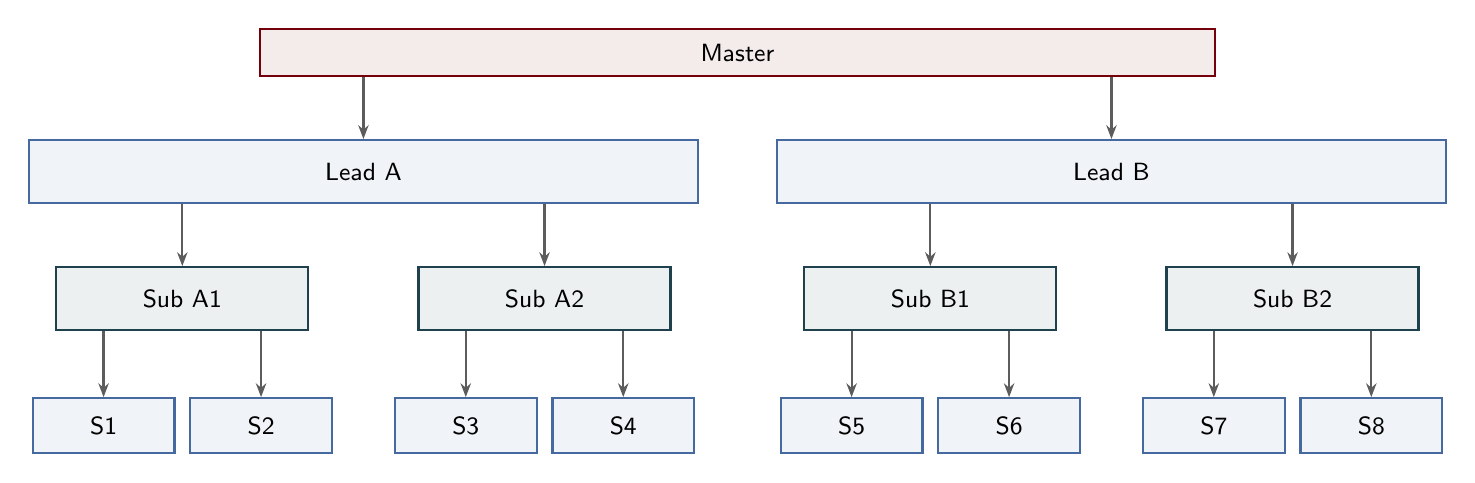
\begin{tikzpicture}[node distance=0.8cm and 0.8cm]
  % Master bar
  \node[agentbox=garnet, minimum width=\textwidth, minimum height=0.6cm] (master) {Master};

  % 2 Leads
  \node[agentbox=atlantic, minimum width=8.5cm] at ([yshift=-1.2cm, xshift=-4.75cm]master.south) (leadA) {Lead A};
  \node[agentbox=atlantic, minimum width=8.5cm] at ([yshift=-1.2cm, xshift=4.75cm]master.south) (leadB) {Lead B};
  \draw[dataarrow] (master.south -| leadA) -- (leadA);
  \draw[dataarrow] (master.south -| leadB) -- (leadB);

  % 4 Sub-leads (2 under each Lead)
  \node[agentbox=congaree, minimum width=3.2cm] at ([yshift=-1.2cm, xshift=-2.3cm]leadA.south) (subA1) {Sub A1};
  \node[agentbox=congaree, minimum width=3.2cm] at ([yshift=-1.2cm, xshift=2.3cm]leadA.south) (subA2) {Sub A2};
  \node[agentbox=congaree, minimum width=3.2cm] at ([yshift=-1.2cm, xshift=-2.3cm]leadB.south) (subB1) {Sub B1};
  \node[agentbox=congaree, minimum width=3.2cm] at ([yshift=-1.2cm, xshift=2.3cm]leadB.south) (subB2) {Sub B2};
  \draw[dataarrow] (leadA.south -| subA1) -- (subA1);
  \draw[dataarrow] (leadA.south -| subA2) -- (subA2);
  \draw[dataarrow] (leadB.south -| subB1) -- (subB1);
  \draw[dataarrow] (leadB.south -| subB2) -- (subB2);

  % 8 Slaves (2 under each Sub-lead)
  \node[workerbox] at ([yshift=-1.2cm, xshift=-1.0cm]subA1.south) (s1) {S1};
  \node[workerbox] at ([yshift=-1.2cm, xshift=1.0cm]subA1.south) (s2) {S2};
  \node[workerbox] at ([yshift=-1.2cm, xshift=-1.0cm]subA2.south) (s3) {S3};
  \node[workerbox] at ([yshift=-1.2cm, xshift=1.0cm]subA2.south) (s4) {S4};
  \node[workerbox] at ([yshift=-1.2cm, xshift=-1.0cm]subB1.south) (s5) {S5};
  \node[workerbox] at ([yshift=-1.2cm, xshift=1.0cm]subB1.south) (s6) {S6};
  \node[workerbox] at ([yshift=-1.2cm, xshift=-1.0cm]subB2.south) (s7) {S7};
  \node[workerbox] at ([yshift=-1.2cm, xshift=1.0cm]subB2.south) (s8) {S8};

  \draw[dataarrow] (subA1.south -| s1) -- (s1);
  \draw[dataarrow] (subA1.south -| s2) -- (s2);
  \draw[dataarrow] (subA2.south -| s3) -- (s3);
  \draw[dataarrow] (subA2.south -| s4) -- (s4);
  \draw[dataarrow] (subB1.south -| s5) -- (s5);
  \draw[dataarrow] (subB1.south -| s6) -- (s6);
  \draw[dataarrow] (subB2.south -| s7) -- (s7);
  \draw[dataarrow] (subB2.south -| s8) -- (s8);
\end{tikzpicture}
\caption{Deep architecture: four layers with hierarchical branching. Master delegates to 2 leads, each lead manages 2 sub-leads, and each sub-lead coordinates 2 slaves. Three sequential handoffs are required to reach execution. Best for complex decomposition requiring hierarchical refinement.}
\label{fig:deep_architecture}
\end{figure*}

\begin{figure*}[t]
\centering
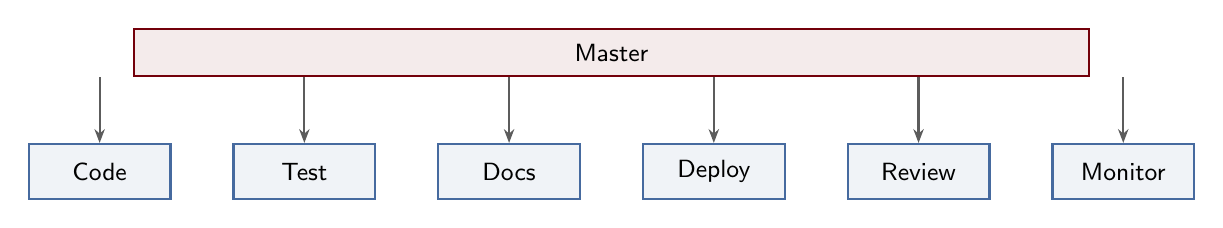
\begin{tikzpicture}[node distance=0.8cm and 0.8cm]
  % Master bar - text width
  \node[agentbox=garnet, minimum width=\textwidth, minimum height=0.6cm] (master) {Master};

  % 6 specialist slaves in one row
  \node[workerbox] at ([yshift=-1.2cm, xshift=-6.5cm]master.south) (code) {Code};
  \node[workerbox] at ([yshift=-1.2cm, xshift=-3.9cm]master.south) (test) {Test};
  \node[workerbox] at ([yshift=-1.2cm, xshift=-1.3cm]master.south) (docs) {Docs};
  \node[workerbox] at ([yshift=-1.2cm, xshift=1.3cm]master.south) (deploy) {Deploy};
  \node[workerbox] at ([yshift=-1.2cm, xshift=3.9cm]master.south) (review) {Review};
  \node[workerbox] at ([yshift=-1.2cm, xshift=6.5cm]master.south) (monitor) {Monitor};

  % Arrows from master to each specialist
  \foreach \s in {code,test,docs,deploy,review,monitor} {
    \draw[dataarrow] (master.south -| \s) -- (\s);
  }
\end{tikzpicture}
\caption{Wide architecture: few layers with broad branching. Six domain specialists operate in parallel, coordinated by a single master. Fewer handoffs mean lower latency. Best for domain coverage requiring specialized expertise.}
\label{fig:wide_architecture}
\end{figure*}

Figures~\ref{fig:deep_architecture} and~\ref{fig:wide_architecture} contrast deep and wide architectures. The deep system on the left requires four sequential handoffs to reach the execution layer. Each handoff adds latency and potential for information loss. The wide system on the right allows six specialists to operate in parallel, coordinated by a single master above them. The visual contrast is stark: depth is tall and narrow, width is short and broad. The choice between them depends on whether your bottleneck is decomposition complexity (which benefits from depth) or domain coverage (which benefits from width).

In practice, successful systems often combine both approaches. A three-layer architecture might have a strategic layer at the top, a planning layer that delegates to domain-specific masters in the middle, and domain specialists at the bottom. The strategic layer goes deep to separate concerns. The domain specialists go wide to cover diverse technical areas. This hybrid structure balances the competing demands of abstraction, specialization, and coordination.


% ── Part VII: Formal Patterns + Selection (Sections 26-31)
%% Sections 26--31: Common Patterns in Multi-Agent Systems
%% This file contains \section commands, figures, and tables for \input into main document

\section{The Pipeline Pattern}\label{sec:pipeline}

The pipeline pattern organizes computation as a strictly sequential chain of transformations.
Each stage receives input from the previous stage, performs a specific transformation, and passes the result to the next stage.
Stages execute one after another---there is no parallelism within the pipeline itself.
The master's role is minimal: it assembles the chain, initiates the first stage, and monitors for failures.

This pattern offers several advantages.
The sequential structure makes pipelines simple to reason about and debug---each intermediate output can be inspected in isolation.
Pipelines naturally fit transformation workflows where each step builds on the previous result: data ingestion, parsing, analysis, formatting, and output.
The clear separation of concerns allows each stage to be developed, tested, and maintained independently.

However, pipelines have inherent limitations.
Total latency is the sum of all stage latencies---no overlap is possible.
A failure at any stage blocks the entire pipeline, requiring careful error handling at each boundary.
For tasks with independent subtasks, the pipeline's strict sequencing wastes potential parallelism.
Despite these constraints, pipelines remain a fundamental building block for workflows that require ordered transformations.

Figure~\ref{fig:patterns_pipe_fan} (top) illustrates a five-stage pipeline for document processing.
Raw input enters the Ingest stage, producing structured data for Parse, which feeds analyzed content to Analyze, then formatted output to Format, and finally the polished result to Output.
The master establishes the chain and monitors each stage, but the data flows strictly left-to-right through the sequence.

\begin{figure*}[t]
\centering
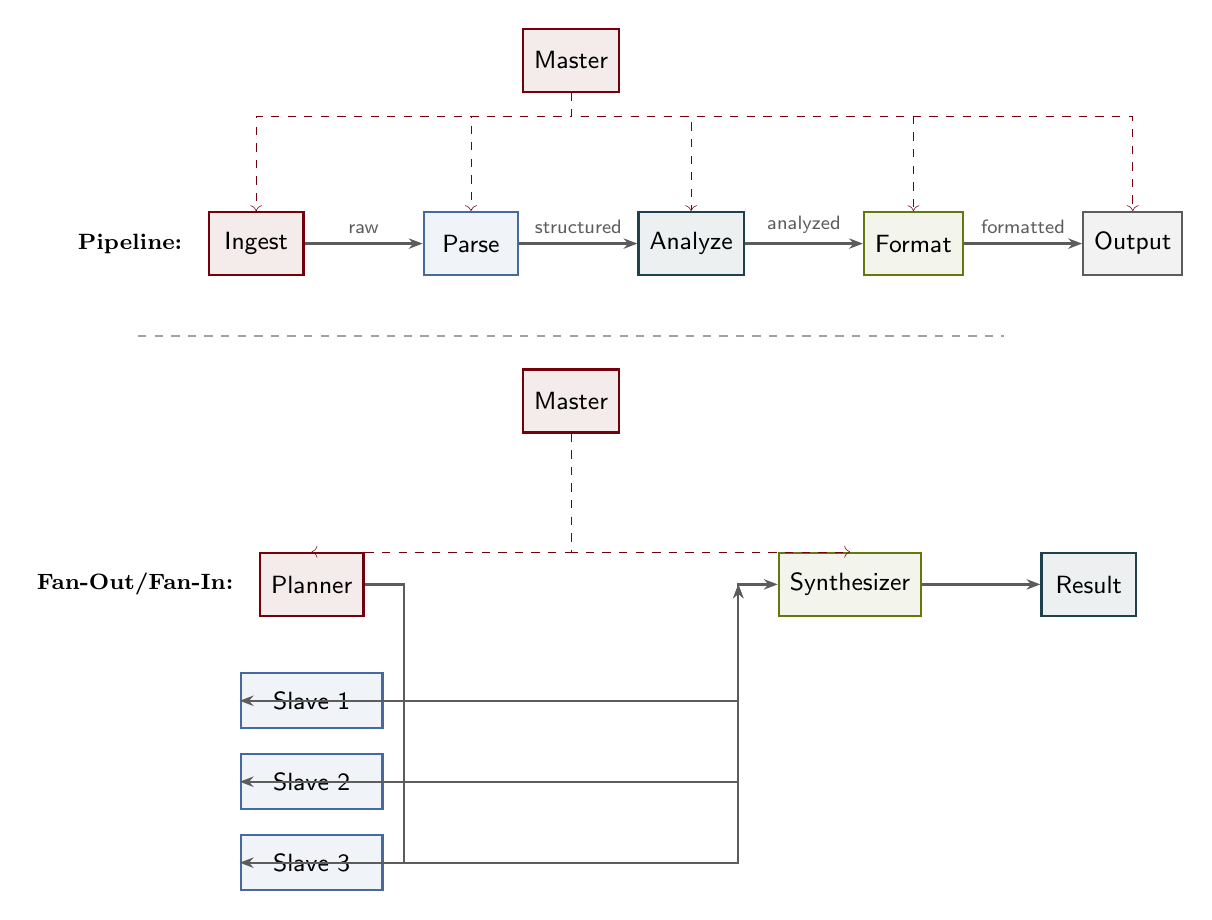
\begin{tikzpicture}[
  node distance=1.2cm and 1.5cm,
  every node/.style={font=\small}
]

% TOP HALF: Pipeline Pattern
\node[agentbox=garnet, minimum width=1.2cm] (orch) {Master};
\node[agentbox=garnet, below=1.5cm of orch, xshift=-4cm, minimum width=1.2cm] (ingest) {Ingest};
\node[agentbox=atlantic, right=of ingest, minimum width=1.2cm] (parse) {Parse};
\node[agentbox=congaree, right=of parse, minimum width=1.2cm] (analyze) {Analyze};
\node[agentbox=horseshoe, right=of analyze, minimum width=1.2cm] (format) {Format};
\node[agentbox=bk70, right=of format, minimum width=1.2cm] (output) {Output};

% Pipeline flow with data labels
\draw[dataarrow] (ingest) -- node[labelnode, above] {raw} (parse);
\draw[dataarrow] (parse) -- node[labelnode, above] {structured} (analyze);
\draw[dataarrow] (analyze) -- node[labelnode, above] {analyzed} (format);
\draw[dataarrow] (format) -- node[labelnode, above] {formatted} (output);

% Master coordination (thin dashed)
\draw[dashed, garnet, very thin, ->] (orch.south) -- ++(0,-0.3) -| (ingest.north);
\draw[dashed, garnet, very thin, ->] (orch.south) -- ++(0,-0.3) -| (parse.north);
\draw[dashed, garnet, very thin, ->] (orch.south) -- ++(0,-0.3) -| (analyze.north);
\draw[dashed, garnet, very thin, ->] (orch.south) -- ++(0,-0.3) -| (format.north);
\draw[dashed, garnet, very thin, ->] (orch.south) -- ++(0,-0.3) -| (output.north);

% Label
\node[left=0.2cm of ingest, font=\footnotesize\bfseries] {Pipeline:};

% SEPARATOR
\draw[dashed, bk50, thick] (-5.5,-3.5) -- (5.5,-3.5);

% BOTTOM HALF: Fan-Out / Fan-In Pattern
\node[agentbox=garnet, below=3.5cm of orch, minimum width=1.2cm] (orch2) {Master};
\node[agentbox=garnet, below left=1.5cm and 2cm of orch2, minimum width=1.2cm] (planner) {Planner};

\node[workerbox, below=1.5cm of planner, yshift=0.8cm] (w1) {Slave 1};
\node[workerbox, below=0.3cm of w1] (w2) {Slave 2};
\node[workerbox, below=0.3cm of w2] (w3) {Slave 3};

\node[agentbox=horseshoe, below right=1.5cm and 2cm of orch2, minimum width=1.2cm] (synth) {Synthesizer};
\node[agentbox=congaree, right=1.5cm of synth, minimum width=1.2cm] (result) {Result};

% Fan-out arrows
\draw[dataarrow] (planner.east) -- ++(0.5,0) |- (w1.west);
\draw[dataarrow] (planner.east) -- ++(0.5,0) |- (w2.west);
\draw[dataarrow] (planner.east) -- ++(0.5,0) |- (w3.west);

% Fan-in arrows
\draw[dataarrow] (w1.east) -| ([xshift=-0.5cm]synth.west) -- (synth.west);
\draw[dataarrow] (w2.east) -| ([xshift=-0.5cm]synth.west);
\draw[dataarrow] (w3.east) -| ([xshift=-0.5cm]synth.west);

% Final result
\draw[dataarrow] (synth) -- (result);

% Master coordination
\draw[dashed, garnet, very thin, ->] (orch2.south) |- (planner.north);
\draw[dashed, garnet, very thin, ->] (orch2.south) |- (synth.north);

% Label
\node[left=0.2cm of planner, font=\footnotesize\bfseries] {Fan-Out/Fan-In:};

\end{tikzpicture}
\caption{%
  \textbf{Top:} The pipeline pattern processes data through a sequential chain of transformations.
  Each stage performs a specific operation and forwards the result to the next stage.
  The master coordinates the chain but does not participate in data transformation.
  \textbf{Bottom:} The fan-out/fan-in pattern distributes independent subtasks to parallel slaves.
  The planner decomposes the problem, slaves execute in parallel, and the synthesizer merges results.
}
\label{fig:patterns_pipe_fan}
\end{figure*}

\section{The Fan-Out/Fan-In Pattern}\label{sec:fanout}

The fan-out/fan-in pattern exploits task parallelism by decomposing work into independent subtasks, executing them concurrently, and merging the results.
A planner examines the overall task, identifies subtasks that can proceed without coordination, and distributes them to a set of parallel slaves.
Each slave executes its subtask independently---no inter-slave communication is required.
A synthesizer collects all slave outputs and combines them into a unified result.

This pattern is ubiquitous in tasks with natural parallelism.
Literature reviews fan out queries to multiple databases or search engines, then synthesize the combined bibliography.
Code reviews fan out file-level analyses to separate slaves, then merge findings.
Testing frameworks fan out test suites to parallel executors, then aggregate pass/fail results.
The key enabling assumption is subtask independence: each slave must be able to complete its work without information from other slaves.

The planner's decomposition step is critical.
If subtasks have hidden dependencies---shared state, ordering constraints, or required coordination---results may be inconsistent or incomplete.
Conversely, correct decomposition yields significant speedup: total latency becomes the maximum slave latency rather than the sum of all subtask latencies.
The pattern also provides natural fault tolerance: if a slave fails, the master can retry that subtask without affecting other slaves.

Figure~\ref{fig:patterns_pipe_fan} (bottom) shows a fan-out/fan-in workflow.
The planner distributes three subtasks to three slaves operating in parallel.
Each slave independently completes its assignment and returns results to the synthesizer, which merges them into a final output.
The master monitors both planning and synthesis but does not participate in subtask execution.

\section{The Master-Slave Pool Pattern}\label{sec:master_slave}

The master-slave pool pattern manages large-scale batch processing through a centralized task queue and a pool of interchangeable slaves.
A master agent maintains the queue, adding tasks as they arrive or as prior results generate new work.
Slaves pull tasks from the queue, execute them, return results to the master, and immediately request the next task.
Slaves are stateless and interchangeable---if one slave fails, another can retry the same task.
The master tracks completion and decides when the queue is empty or a stopping condition is met.

This pattern excels at throughput-oriented workflows.
Analyzing thousands of log files, running extensive test suites, processing batches of data records, or generating multiple variations of a design all fit naturally into the master-slave model.
The pool size can scale dynamically: add slaves to increase throughput, remove slaves when load decreases.
The master can implement sophisticated scheduling policies: prioritize high-value tasks, load-balance across slaves, or retry failed tasks with backoff.

The iterative nature distinguishes this pattern from simple fan-out.
The master may add new tasks to the queue based on results from completed tasks, creating a feedback loop.
For example, a web crawler's master enqueues initial seed URLs; as slaves fetch pages, they report discovered links, which the master adds to the queue.
This dynamic task generation continues until no new work is discovered or a resource limit is reached.

Figure~\ref{fig:patterns_pool_feedback} (top) illustrates the master-slave pool.
The master enqueues tasks \texttt{T1}, \texttt{T2}, \texttt{T3}, \texttt{T4}, and so on into a central queue.
Four slaves dequeue tasks, execute them, and return results to the master.
The master can dynamically add new tasks based on those results, creating an iterative workflow.

\begin{figure*}[t]
\centering
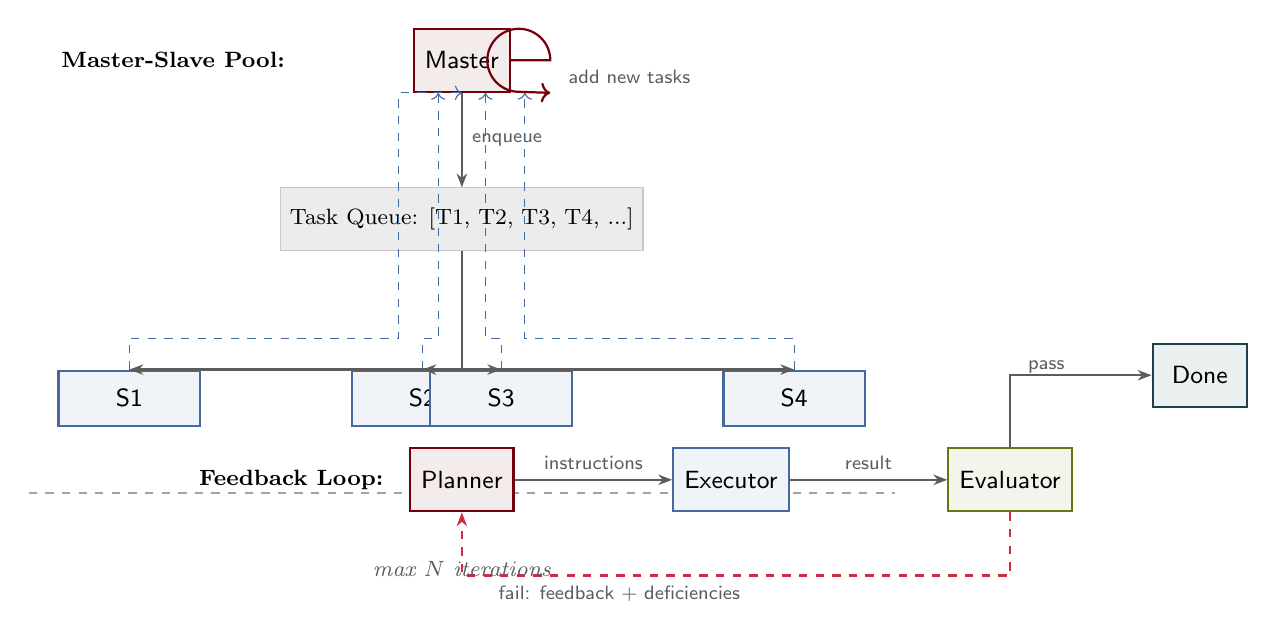
\begin{tikzpicture}[
  node distance=1.2cm and 1.5cm,
  every node/.style={font=\small}
]

% TOP HALF: Master-Slave Pool Pattern
\node[agentbox=garnet, minimum width=1.2cm] (master) {Master};
\node[draw=bk30, fill=bk10, below=1.2cm of master, minimum width=3.5cm, minimum height=0.8cm, font=\footnotesize] (queue) {Task Queue: [T1, T2, T3, T4, ...]};

\node[workerbox, below left=1.5cm and 1cm of queue] (w1) {S1};
\node[workerbox, below=1.5cm of queue, xshift=-0.5cm] (w2) {S2};
\node[workerbox, below=1.5cm of queue, xshift=0.5cm] (w3) {S3};
\node[workerbox, below right=1.5cm and 1cm of queue] (w4) {S4};

% Enqueue
\draw[dataarrow] (master.south) -- node[labelnode, right] {enqueue} (queue.north);

% Dequeue
\draw[dataarrow] (queue.south) |- (w1.north);
\draw[dataarrow] (queue.south) |- (w2.north);
\draw[dataarrow] (queue.south) |- (w3.north);
\draw[dataarrow] (queue.south) |- (w4.north);

% Results back to master (dashed)
\draw[dashed, atlantic, ->] (w1.north) -- ++(0,0.4) -| ([xshift=-0.8cm]master.south) -- (master.south);
\draw[dashed, atlantic, ->] (w2.north) -- ++(0,0.4) -| ([xshift=-0.3cm]master.south);
\draw[dashed, atlantic, ->] (w3.north) -- ++(0,0.4) -| ([xshift=0.3cm]master.south);
\draw[dashed, atlantic, ->] (w4.north) -- ++(0,0.4) -| ([xshift=0.8cm]master.south);

% Loop arrow on master
\draw[->, garnet, thick] (master.east) -- ++(0.5,0) arc[start angle=0, end angle=270, radius=0.4cm] -- ([xshift=0.5cm]master.south east) node[labelnode, right, xshift=0.1cm, yshift=0.2cm] {add new tasks};

% Label
\node[left=1.5cm of master, font=\footnotesize\bfseries] {Master-Slave Pool:};

% SEPARATOR
\draw[dashed, bk50, thick] (-5.5,-5.5) -- (5.5,-5.5);

% BOTTOM HALF: Feedback Loop Pattern
\node[agentbox=garnet, below=4.5cm of master, minimum width=1.2cm] (planner2) {Planner};
\node[agentbox=atlantic, right=2cm of planner2, minimum width=1.2cm] (executor) {Executor};
\node[agentbox=horseshoe, right=2cm of executor, minimum width=1.2cm] (evaluator) {Evaluator};

\node[agentbox=congaree, above right=0.5cm and 1cm of evaluator, minimum width=1.2cm] (done) {Done};

% Forward flow
\draw[dataarrow] (planner2) -- node[labelnode, above] {instructions} (executor);
\draw[dataarrow] (executor) -- node[labelnode, above] {result} (evaluator);

% Pass branch
\draw[dataarrow] (evaluator.north) |- node[labelnode, above right, xshift=0.1cm, yshift=-0.1cm] {pass} (done.west);

% Fail branch (feedback loop)
\draw[dataarrow=rose, dashed] (evaluator.south) -- ++(0,-0.8) -| node[labelnode, below, xshift=2cm] {fail: feedback + deficiencies} (planner2.south);

% Iteration label
\node[labelnode, below=0.5cm of planner2, font=\footnotesize\itshape] {max $N$ iterations};

% Label
\node[left=0.2cm of planner2, font=\footnotesize\bfseries] {Feedback Loop:};

\end{tikzpicture}
\caption{%
  \textbf{Top:} The master-slave pool pattern uses a centralized task queue and stateless slaves.
  The master enqueues tasks, slaves dequeue and execute them, and results flow back to the master.
  The master can add new tasks based on results, enabling iterative workflows.
  \textbf{Bottom:} The feedback loop pattern refines results through iterative execution.
  The planner issues instructions, the executor produces a result, the evaluator judges quality, and failures trigger revised planning with feedback about deficiencies.
}
\label{fig:patterns_pool_feedback}
\end{figure*}

\section{The Feedback Loop Pattern}\label{sec:feedback}

The feedback loop pattern addresses tasks where initial attempts rarely achieve acceptable quality.
Results from execution flow back to a planning agent for iterative refinement.
The planner issues instructions, an executor produces a result, an evaluator judges quality, and failures trigger revised planning informed by specific deficiencies.
This cycle continues until quality is sufficient or a maximum iteration count is reached.

Bidirectional communication between planner and executor distinguishes this pattern from simple retry logic.
The evaluator does not merely return pass/fail---it provides detailed feedback about what went wrong, which aspects need improvement, and which constraints were violated.
The planner uses this feedback to adjust its next set of instructions, focusing on the identified deficiencies rather than starting from scratch.

Common applications include code generation (write code, run tests, fix failures, repeat), document writing (draft text, review for clarity and accuracy, revise weak sections), and optimization (measure performance, identify bottlenecks, adjust parameters, re-measure).
In each case, the first attempt provides valuable information that guides subsequent refinement.

The feedback loop's iterative nature has cost implications.
Each iteration consumes tokens for planning, execution, and evaluation.
Setting appropriate stopping conditions is critical: too few iterations may yield poor quality, while too many waste resources on diminishing returns.
Effective evaluators provide actionable feedback that enables rapid convergence, reducing the total iteration count needed.

Figure~\ref{fig:patterns_pool_feedback} (bottom) shows the feedback loop structure.
The planner sends instructions to the executor, which produces a result for the evaluator.
If the evaluator judges the result acceptable, the workflow terminates.
Otherwise, the evaluator returns detailed feedback to the planner, which incorporates those deficiencies into revised instructions for the next iteration.

\section{Combining Patterns}\label{sec:combining}

Real systems rarely use a single pattern in isolation.
Complex workflows compose multiple patterns, each handling a phase suited to its strengths.
A research pipeline might use fan-out for literature search, a sequential pipeline for data cleaning, a master-slave pool for running experiments, and feedback loops for manuscript writing.
The master at the top selects and coordinates the appropriate pattern for each phase based on the task structure.

The key design principle is matching the pattern to the task's inherent characteristics.
Tasks with independent subtasks benefit from fan-out parallelism.
Sequential transformations where each step depends on the previous result require a pipeline.
Iterative refinement toward a quality target needs a feedback loop.
Large-scale batch processing with uniform work items calls for a master-worker pool.
By analyzing task dependencies, ordering constraints, quality requirements, and scale, designers can select the pattern that best exploits the task structure.

Composition requires careful boundary management.
Outputs from one pattern become inputs to the next, requiring compatible data formats and error-handling conventions.
The top-level master manages these transitions, ensuring that failures in one pattern do not silently propagate to dependent patterns.
State management becomes critical: which pattern owns intermediate results, how are they cached or persisted, and who is responsible for cleanup.

Hybrid workflows also enable adaptive execution.
The master can monitor pattern performance and switch strategies dynamically.
A fan-out phase that discovers subtask dependencies might transition to a pipeline.
A pipeline stage that encounters a large batch might spawn a master-slave pool for that stage alone.
This flexibility allows systems to respond to workload characteristics discovered at runtime.

Figure~\ref{fig:composite_workflow} illustrates a composite research workflow.
The top-level research master coordinates four phases, each using a different pattern.
The literature phase fans out queries to multiple sources and merges results.
The data phase pipelines ingestion, cleaning, and validation.
The experiment phase uses a master-slave pool to run many trials in parallel.
The writing phase employs a feedback loop to iteratively draft and revise the manuscript.

\begin{figure*}[t]
\centering
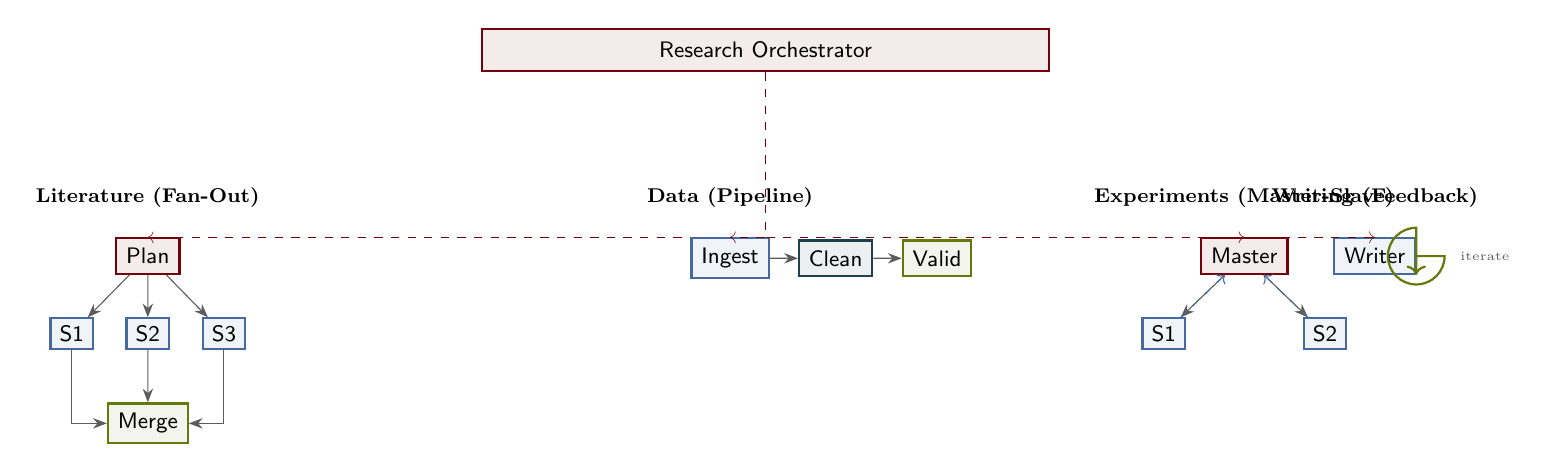
\begin{tikzpicture}[
  node distance=0.8cm and 1.5cm,
  every node/.style={font=\footnotesize},
  scale=0.9, transform shape
]

% Top orchestrator (wide)
\node[agentbox=garnet, minimum width=8cm, minimum height=0.6cm] (top) {Research Orchestrator};

% Branch 1: Literature (Fan-Out)
\node[below left=1.5cm and 3cm of top, font=\footnotesize] (lit_label) {\textbf{Literature (Fan-Out)}};
\node[agentbox=garnet, below=0.3cm of lit_label, minimum width=0.8cm, minimum height=0.5cm] (lit_plan) {Plan};
\node[workerbox, below left=0.6cm and 0.3cm of lit_plan, minimum width=0.6cm, minimum height=0.4cm] (w1) {S1};
\node[workerbox, below=0.6cm of lit_plan, minimum width=0.6cm, minimum height=0.4cm] (w2) {S2};
\node[workerbox, below right=0.6cm and 0.3cm of lit_plan, minimum width=0.6cm, minimum height=0.4cm] (w3) {S3};
\node[agentbox=horseshoe, below=1.8cm of lit_plan, minimum width=0.8cm, minimum height=0.5cm] (merge) {Merge};

\draw[dataarrow, thin] (lit_plan) -- (w1);
\draw[dataarrow, thin] (lit_plan) -- (w2);
\draw[dataarrow, thin] (lit_plan) -- (w3);
\draw[dataarrow, thin] (w1) |- (merge);
\draw[dataarrow, thin] (w2) -- (merge);
\draw[dataarrow, thin] (w3) |- (merge);
\draw[dashed, garnet, very thin, ->] (top.south) |- (lit_plan.north);

% Branch 2: Data (Pipeline)
\node[below=1.5cm of top, xshift=-0.5cm, font=\footnotesize] (data_label) {\textbf{Data (Pipeline)}};
\node[agentbox=atlantic, below=0.3cm of data_label, minimum width=0.7cm, minimum height=0.5cm] (d1) {Ingest};
\node[agentbox=congaree, right=0.4cm of d1, minimum width=0.7cm, minimum height=0.5cm] (d2) {Clean};
\node[agentbox=horseshoe, right=0.4cm of d2, minimum width=0.7cm, minimum height=0.5cm] (d3) {Valid};

\draw[dataarrow, thin] (d1) -- (d2);
\draw[dataarrow, thin] (d2) -- (d3);
\draw[dashed, garnet, very thin, ->] (top.south) |- (d1.north);

% Branch 3: Experiments (Master-Slave)
\node[below right=1.5cm and 0.5cm of top, font=\footnotesize] (exp_label) {\textbf{Experiments (Master-Slave)}};
\node[agentbox=garnet, below=0.3cm of exp_label, minimum width=0.8cm, minimum height=0.5cm] (exp_master) {Master};
\node[workerbox, below left=0.6cm and 0.2cm of exp_master, minimum width=0.6cm, minimum height=0.4cm] (e1) {S1};
\node[workerbox, below right=0.6cm and 0.2cm of exp_master, minimum width=0.6cm, minimum height=0.4cm] (e2) {S2};

\draw[dataarrow, thin] (exp_master) -- (e1);
\draw[dataarrow, thin] (exp_master) -- (e2);
\draw[dashed, atlantic, thin, ->] (e1) -- (exp_master);
\draw[dashed, atlantic, thin, ->] (e2) -- (exp_master);
\draw[dashed, garnet, very thin, ->] (top.south) |- (exp_master.north);

% Branch 4: Writing (Feedback)
\node[below right=1.5cm and 3cm of top, font=\footnotesize] (write_label) {\textbf{Writing (Feedback)}};
\node[agentbox=atlantic, below=0.3cm of write_label, minimum width=0.8cm, minimum height=0.5cm] (writer) {Writer};

\draw[->, horseshoe, thick] (writer.east) -- ++(0.4,0) arc[start angle=0, end angle=-270, radius=0.4cm] -- (writer.south east);
\node[labelnode, right=0.5cm of writer, font=\tiny] {iterate};
\draw[dashed, garnet, very thin, ->] (top.south) |- (writer.north);

\end{tikzpicture}
\caption{%
  A composite research workflow combines four patterns under a single master.
  The literature phase uses fan-out to query multiple sources in parallel.
  The data phase pipelines ingestion, cleaning, and validation steps.
  The experiment phase employs a master-slave pool for high-throughput execution.
  The writing phase uses a feedback loop to iteratively refine the manuscript.
  Each pattern handles the phase best suited to its strengths.
}
\label{fig:composite_workflow}
\end{figure*}

\section{Pattern Selection Guide}\label{sec:selection}

Choosing the right pattern---or combination of patterns---requires analyzing the task structure along several dimensions.
Are subtasks independent, or does each depend on results from others?
Must steps execute in a specific order, or can they run concurrently?
Is iteration needed to achieve acceptable quality?
Is the workload large and uniform, or small and varied?

Independent subtasks with no ordering constraints favor fan-out/fan-in parallelism.
If subtasks must execute sequentially---each transforming the output of the previous stage---a pipeline is appropriate.
Tasks requiring iterative refinement call for a feedback loop, where each iteration incorporates lessons from prior attempts.
Large-scale batch processing with uniform work items benefits from a master-slave pool, which maximizes throughput through dynamic load balancing.

Table~\ref{tab:selection_guide} summarizes these considerations across seven dimensions.
Task independence indicates whether subtasks can execute without coordination.
Iteration captures whether quality improvement requires multiple passes.
Scale reflects the typical number of subtasks: pipelines handle a few stages, fan-out manages moderate parallelism, and master-slave pools scale to hundreds of tasks.
Quality emphasis distinguishes patterns optimized for throughput (master-slave) from those focused on refinement (feedback loop).

Token cost varies by pattern.
Pipelines incur linear cost proportional to the number of stages.
Fan-out patterns pay for subtasks in parallel but avoid duplication.
Master-worker pools consume tokens proportional to the total workload.
Feedback loops multiply costs by the number of iterations, making early convergence critical.

Complexity reflects both implementation difficulty and cognitive load during debugging.
Pipelines are simplest to implement and reason about.
Fan-out and master-slave patterns add coordination overhead.
Feedback loops require careful evaluator design and stopping logic.

Latency characteristics also differ.
Pipeline latency is the sum of all stage latencies.
Fan-out latency is determined by the slowest worker.
Master-slave pools batch tasks, trading some latency for throughput.
Feedback loops multiply latency by iteration count.

The final row, ``Best for,'' summarizes canonical use cases.
Pipelines excel at sequential transformations.
Fan-out handles independent parallel work.
Master-slave pools optimize batch processing.
Feedback loops enable iterative refinement toward quality targets.

By evaluating a task against these dimensions, designers can systematically select the pattern that best matches the task structure.

\begin{table*}[t]
\centering
\caption{Pattern selection guide based on task characteristics.}
\label{tab:selection_guide}
\small
\begin{tabularx}{\textwidth}{l X X X X}
\toprule
\textbf{Criterion} & \textbf{Pipeline} & \textbf{Fan-Out/Fan-In} & \textbf{Master-Slave} & \textbf{Feedback Loop} \\
\midrule
Task independence & Low & High & High & Low \\
Iteration needed & No & No & Optional & Yes \\
Scale (subtasks) & 3--5 & 3--20 & 10--100+ & 2--5 \\
Quality emphasis & Moderate & Moderate & Throughput & High \\
Token cost & Linear & Parallel & High & Moderate \\
Complexity & Low & Medium & Medium & Medium \\
Latency & Sum of stages & Max of workers & Batched & Iterations $\times$ stage \\
Best for & Transforms & Independent work & Batch processing & Refinement \\
\bottomrule
\end{tabularx}
\end{table*}

Figure~\ref{fig:taxonomy} places these patterns within a broader taxonomy of agent architectures.
At the top level, architectures divide into single-agent and multi-agent categories.
Single-agent systems may operate in streaming, batch, or parallel modes, but they lack the coordination mechanisms that define multi-agent patterns.

Multi-agent systems further divide into flat and hierarchical organizations.
Flat architectures distribute control: no agent has authority over others.
The pipeline and fan-out/fan-in patterns are flat---the master coordinates but does not command.
Hierarchical architectures establish explicit control relationships.
Master-slave pools and feedback loops are hierarchical---the master or planner directs subordinate agents.

This taxonomy provides a roadmap for navigating design space.
Starting from the task characteristics, designers first decide single-agent versus multi-agent, then flat versus hierarchical, and finally select the specific pattern that best fits the task structure.

\begin{figure*}[t]
\centering
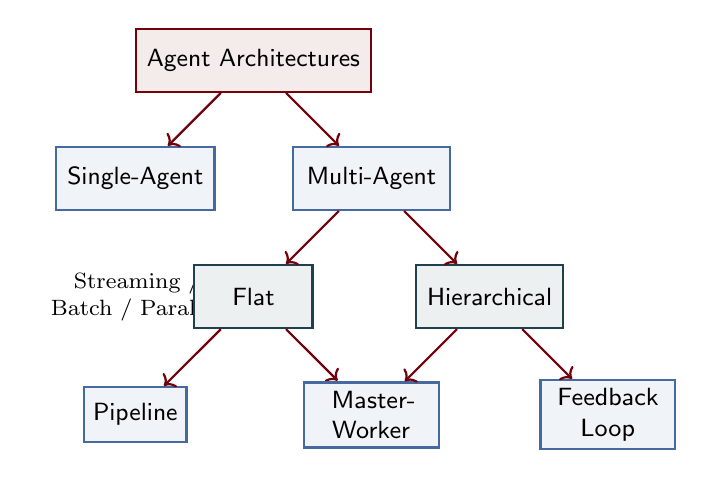
\begin{tikzpicture}[
  level distance=1.5cm,
  sibling distance=3cm,
  edge from parent/.style={draw, garnet, thick, ->},
  every node/.style={font=\small}
]

\node[agentbox=garnet, minimum width=2.5cm] {Agent Architectures}
  child {
    node[agentbox=atlantic, minimum width=2cm] {Single-Agent}
    child {
      node[font=\footnotesize, text width=2.5cm, align=center] {Streaming / Batch / Parallel}
      edge from parent[draw=none]
    }
  }
  child {
    node[agentbox=atlantic, minimum width=2cm] {Multi-Agent}
    child {
      node[agentbox=congaree, minimum width=1.5cm] {Flat}
      child {
        node[workerbox, minimum width=1.3cm] {Pipeline}
      }
      child {
        node[workerbox, minimum width=1.3cm, text width=1.5cm, align=center] {Fan-Out/\\Fan-In}
      }
    }
    child {
      node[agentbox=congaree, minimum width=1.5cm] {Hierarchical}
      child {
        node[workerbox, minimum width=1.3cm, text width=1.5cm, align=center] {Master-\\Worker}
      }
      child {
        node[workerbox, minimum width=1.3cm, text width=1.5cm, align=center] {Feedback\\Loop}
      }
    }
  };

\end{tikzpicture}
\caption{%
  A taxonomy of agent architectures.
  Single-agent systems may operate in streaming, batch, or parallel modes but lack multi-agent coordination.
  Multi-agent systems divide into flat (pipeline, fan-out/fan-in) and hierarchical (master-worker, feedback loop) organizations.
  This taxonomy provides a structured approach to pattern selection based on control flow and task structure.
}
\label{fig:taxonomy}
\end{figure*}


% ── Conclusion ────────────────────────────────────────────
\section{Conclusion}\label{sec:conclusion}

We have traced a deliberate path from the simplest computational unit—an LLM as a text-in, text-out function—to increasingly sophisticated multi-agent systems. This journey did not require changing the LLM itself. Instead, we progressively wrapped the core model in layers of control: first with agents that observe and act, then with execution models that orchestrated parallel and streaming invocations, next with sub-agent hierarchies that decomposed complex problems, and finally with orchestration patterns that coordinated multiple independent systems. At each step, the model remained constant while the architecture around it grew in complexity and capability.

This insight is fundamental: the LLM is an uncommitted tool. Its power comes not from its individual inference but from how we compose multiple inferences within a structured process. The four canonical patterns we examined—pipeline, fan-out/fan-in, master-slave, and feedback loop—are the vocabulary of this composition. These patterns are not LLM-specific inventions; they echo classical concurrent and distributed computing. Their importance here is that they are small enough to understand completely, composable enough to combine into larger systems, and general enough to apply across an enormous range of agent tasks. A system that orchestrates document analysis, code review, or scientific hypothesis testing may use these same patterns, differing only in the details of task decomposition and resource constraints.

Selecting the right architecture is not primarily a question of model capability. Given a task, the architecture emerges from the task's structure: its inherent parallelism, its feedback requirements, its hierarchical depth, and the latency constraints we impose. A well-designed agent system for real-time reasoning may use tight feedback loops and shallow hierarchies. A batch system for asynchronous analysis may embrace deep pipelines and wide fan-outs. Neither choice is superior; each is the natural fit to its problem. This decoupling between model selection and architectural design frees practitioners to reason about systems clearly.

As LLM-based applications move from research prototypes to production systems at scale, these patterns will become foundational. We can already see them emerging in production orchestration frameworks and multi-agent platforms. Understanding them deeply—not merely as abstract diagrams but as concrete execution models with resource, latency, and consistency implications—is essential for anyone building intelligent systems. The progression we have outlined, from simple agents to complex hierarchies, provides both a map and a toolkit for that future. The LLM remains at the heart of the system, but the architecture around it is where the real engineering begins.


\end{document}
